\documentclass[11pt,a4paper]{report}
%%%%%%%%%%%%%%%%%%%%%%%%%%%%%%%%%%%%%%%%%%%%%%%%%%%%%%%%%%%%%%%%%%%%%
%%                                                                 %%
%%    Header file for the Phi-S-X Series                           %%
%%                                                                 %%
%%    german version header_gm.tex is derived from header.tex      %%
%%    by uncommenting the line ``\setboolean{german}{true}'' below %%
%%                                                                 %%
%%    Never edit the german version! all changes must be done      %%
%%    in the english version header.tex                            %%
%%                                                                 %%
%%%%%%%%%%%%%%%%%%%%%%%%%%%%%%%%%%%%%%%%%%%%%%%%%%%%%%%%%%%%%%%%%%%%%
%%%%%%%%%%%%%%%%%%%%%%%%%%%%%%%%%%%%%%%%%%%%%%%%%%%%%%%%%%%%%%%%%%%%%
%%                                                                 %%
%%    Header file for the Phi-S-X Series                           %%
%%                                                                 %%
%%    german version header_gm.tex is derived from header.tex      %%
%%    by uncommenting the line ``\setboolean{german}{true}'' below %%
%%                                                                 %%
%%    Never edit the german version! all changes must be done      %%
%%    in the english version header.tex                            %%
%%                                                                 %%
%%%%%%%%%%%%%%%%%%%%%%%%%%%%%%%%%%%%%%%%%%%%%%%%%%%%%%%%%%%%%%%%%%%%%
%====================================================================
%-- define flag for language adaptations
\usepackage{ifthen}   % allows to select only certain text
\provideboolean{german}
\setboolean{german}{false}
%\setboolean{german}{true}  % uncomment this line for german editions
%====================================================================
%
% Textschriftart: Computer modern Bright
% body:            CM-Bright 10pt
% section titles:  CM-Bright Bold
% formulas:        CM-Bright Math Oblique
%
\usepackage[standard-baselineskips]{cmbright}
\usepackage{cmbright}
\usepackage[T1]{fontenc}
\def\usedfonts{CM-Bright}
\usepackage{typearea}
%\typearea[current]{calc} % benutzt die aktuelle 
       % bindekorrektur (BCOR angabe als parameter in koma usepackage)
       % und berechnet satzspiegel neu
\typearea[current]{11} %fixed div value

\usepackage{textcomp} % special symbols
\usepackage{amsfonts} % special symols
                      % see ftp://ftp.ams.org/pub/tex/doc/amsfonts/amsfndoc.pdf
\usepackage{amssymb}  % CM-Bright provides the AMS symbols
\usepackage{exscale}  % allows to scale math expressions to big fonts, 
                      % e.g. \Huge
\usepackage{curves}
\usepackage{braket}
\usepackage{miller}     % miller indices
\usepackage{chemmacros} % http://www.mychemistry.eu/mychemistry/
\usepackage[numbers]{natbib}     % bibliography style
\usepackage{url}\urlstyle{tt}
\usepackage{float}
\usepackage{bm}       % provides the command \bm{} that makes bold math symbols
\usepackage{amsmath}
\usepackage{amsbsy}   % allows bold mathematical symbols
\usepackage{amscd}
 \usepackage{a4wide}  % it is better to use the ``geometry'' package
\usepackage{array}    % 
\usepackage{fancyhdr} %  defines pagestyle fancy
\usepackage{epsfig}   % include graphics with epsfig
\usepackage{graphicx} % includegraphics
\usepackage{epstopdf}
\usepackage{wrapfig}
\usepackage{fancybox} % allows shadow-boxes
\usepackage{color}    % allows to use color in the text
%\usepackage{eepic}
\usepackage{flafter}  % places picture next to its reference
\usepackage{makeidx}  % make an index
%\usepackage{MnSymbol}  % 
%\usepackage{marvosym}  % 
\usepackage{textcase}
\usepackage{ulem} % defines strikeout \sout{}; underline \uline{}
                  % double underline \uuline{}; wave underline \uwave{}
                  % cross out \xout{}
%
%==========================================================================
%==  page layout  =========================================================
%==========================================================================
% eqnarray environment: reduce with of space in place of each ``&''
\setlength\arraycolsep{1.4pt}
\pagestyle{fancy}
%\renewcommand{\chaptermark}[1]{\markboth{\thechapter\ #1}{}}
\renewcommand{\chaptermark}[1]{\markboth{\MakeUppercase{\thechapter\ #1}}{}}
\fancyhf{} 
\fancyhead[LE]{\textsc{\thepage}\qquad\textsc{\leftmark}}
\fancyhead[RO]{\textsc{\leftmark}\qquad\textsc{\thepage}}
\renewcommand{\headrulewidth}{0.5pt}
\renewcommand{\footrulewidth}{0pt} 
\addtolength{\headheight}{2.5pt}
\fancypagestyle{plain}{\fancyhead{}
   \renewcommand{\headrulewidth}{0pt}
   \fancyfoot[CO]{\bfseries\thepage}}

% Line spacing -----------------------------------------------------------
\newlength{\defbaselineskip}
\setlength{\defbaselineskip}{\baselineskip}
\newcommand{\setlinespacing}[1]%
           {\setlength{\baselineskip}{#1 \defbaselineskip}}
\newcommand{\doublespacing}{\setlength{\baselineskip}%
                           {2.0 \defbaselineskip}}
\newcommand{\singlespacing}{\setlength{\baselineskip}{\defbaselineskip}}

% Absatz einr\"ucken ------------------------------------------------------
%\setlength{\parindent}{0pt}
\setlength{\parskip}{2pt}
% -------------------------------------------------------------------------
\ifthenelse{\boolean{german}}
  {\def\figurename{Abb.}}
  {\def\figurename{Fig.}}
%--------------------------------------------------------------------------
\renewcommand{\arraystretch}{1.15}  % skaliert den Zeilen abstand in der 
    % tabular und array umgebung
%
%==========================================================================
%==  boxes etc ============================================================
%==========================================================================
%== minipage in a shadowbox ===============================================
\newenvironment{myshadowminipage}[1]%
  {\par\noindent\begin{Sbox}\begin{minipage}{\linewidth}\vspace{0.1cm}\begin{center}\uppercase{#1}\end{center}}%
  {\vspace{0.1cm}\end{minipage}\end{Sbox}\shadowbox{\TheSbox}}
%
%== minipage in a framedbox ===============================================
\newenvironment{myframedminipage}%
  {\par\noindent\begin{Sbox}\begin{minipage}\linewidth\vspace{0.1cm}}%
  {\vspace{0.1cm}\end{minipage}\end{Sbox}\fbox{\TheSbox}}
%
\newcommand{\myshadowbox}[1]{\noindent\shadowbox{\parbox{\linewidth}{\smallskip #1\smallskip}}}
\newcommand{\myfbox}[1]{\noindent\fbox{\parbox{\linewidth}{\smallskip #1\smallskip}}\medskip}
%== minipage in a framedbox ===============================================
\newtheorem{defi}{Definition}[chapter]
\newenvironment{definition}[1]%
  {\par\noindent\begin{Sbox}\begin{minipage}{\linewidth}\vspace{0.1cm}\begin{defi}\uppercase{#1}\\\vspace{0.1cm}}%
  {\vspace{0.1cm}\end{defi}\end{minipage}\end{Sbox}\shadowbox{\TheSbox}}
%
%=========================================================================
% color used to point out information to the teacher
\definecolor{highlight}{rgb}{1.0,0.7,0.}
\newcommand{\Special}[1]{\textbf{\textcolor{highlight}{#1}}}
%=========================================================================
%  switch certain parts on and off. uses ifthen package
\newboolean{teacher}\setboolean{teacher}{false}
% this parameter can be changed in the manuscript again
\setboolean{teacher}{true} %private version if true!
\newcommand{\teacheronly}[1]{\ifthenelse{\boolean{teacher}}{#1\hfill\\ }}
\newcommand{\editor}[1]{\textcolor{blue}{\texttt{Editor: #1}}}
\newcommand{\MARK}[1]{\textcolor{blue}{#1}} 
\newcommand{\RED}[1]{\textcolor{red}{#1}} 
%
%==========================================================================
%==  define new symbols                                                 ===
%==========================================================================
% define \stat (stationary state) as an operator like \min
\DeclareMathOperator*{\stat}{stat}
\let\Vec=\mathbold   % cmbright.sty provides a bold/italic math alphabet
\let\Dot=\mathbold   % cmbright.sty provides a bold/italic math alphabet
\let\Ddot=\mathbold   % cmbright.sty provides a bold/italic math alphabet
%
\newcommand{\e}[1]{\mathrm{e}^{#1}}% exponential function
\renewcommand{\Re}{\mathrm{Re}}    % real part
\renewcommand{\Im}{\mathrm{Im}}    % imaginary part
\newcommand{\lagr}{\ell}           % Lagrange dichte
\newcommand{\Lagr}{\mathcal{L}}    % Lagrange Funktion
\newcommand{\erf}{{\rm erf}}       %
\newcommand{\atan}{{\rm atan}}     % arcus tangens
\newcommand{\mat}[1]{\bm{#1}}  % Matrix
\newcommand{\gmat}[1]{{\boldsymbol #1}}  % Matrix(symbol)
\newcommand{\defas}{\stackrel{\text{def}}{=}}  %  is defined as
\ifthenelse{\boolean{german}}
  {\newcommand{\rot}{{\rm\bf rot}}}    % curl
  {\newcommand{\rot}{{\rm\bf curl}}}   % curl
\newcommand{\sgn}{{\rm sgn}}       % sign
\ifthenelse{\boolean{german}}
   {\newcommand{\Tr}{\mathrm{Sp}}}      % trace
   {\newcommand{\Tr}{\mathrm{Tr}}}      % trace
\ifthenelse{\boolean{german}}
   {\newcommand{\grmn}[2]{\footnote{``#2'' hei{\ss}t in englisch ``#1''}}}
   {\newcommand{\grmn}[2]{\footnote{``#1'' translates as ``#2'' into German}}}
% define the equation reference
\ifthenelse{\boolean{german}}
   {\newcommand{\eq}[1]{\text{Gl.}~\ref{#1}}}
   {\newcommand{\eq}[1]{\text{Eq.}~\ref{#1}}}
% define a relation with an equation number ontop
\newcommand{\eqrel}[2]{\stackrel{\eq{#1}}{#2}}
\newcommand{\zero}{\varnothing}
%\newcommand{\ket}[1]{|#1\rangle} % contained in package braket
\newcommand{\sumint}{\int\hspace{-15pt}\sum}
\newcommand{\marker}[1]{\textcolor{blue}{\emph{#1}}}
\renewcommand*{\dot}[1]{\overset{\mbox{\large\bfseries .}}{#1}}
\renewcommand*{\ddot}[1]{\overset{\mbox{\large\bfseries\hspace{+0.1ex}.\hspace{-0.1ex}.}}{#1}}
%
%==========================================================================
%==                                                                     ===
%==========================================================================
% Prevent figures from appearing on a page by themselves
% from http://dcwww.camd.dtu.dk/~schiotz/comp/LatexTips/LatexTips.html
\renewcommand{\topfraction}{0.85}
\renewcommand{\textfraction}{0.1}
\renewcommand{\floatpagefraction}{0.75}
%
%==========================================================================
%==                                                                     ===
%==========================================================================
\makeindex    % make index. uses makeidx package.

%== allow links between documents ============================================
\usepackage{xr}
\usepackage{xr-hyper}
%==  hyperref package (must be last package)
\usepackage[colorlinks=true]{hyperref} %specify this as last package
\hypersetup{citecolor=blue}
\hypersetup{menucolor=magenta}
\hypersetup{urlcolor=blue}      % 
\hypersetup{filecolor=green}    % file links
\hypersetup{linkcolor=magenta}  %table of contents
\hypersetup{pdfauthor={Peter E. Bl\"ochl}}
\hypersetup{pdfdisplaydoctitle=true}
\externaldocument[phisx1-]{/Users/ptpb/Tree/PhiSX/ClassicalMechanics/Book/cm-gm}
\externaldocument[phisx2-]{/Users/ptpb/Tree/PhiSX/Electrodynamics/Book/el-gm}
\externaldocument[phisx3-]{/Users/ptpb/Tree/PhiSX/QuantumMechanics/Book/qm}
\externaldocument[phisx4-]{/Users/ptpb/Tree/PhiSX/StatisticalMechanics/Book/sm}
\externaldocument[phisxqm2-]{/Users/ptpb/Tree/PhiSX/QuantumMechanicsII/Book/qm2}
\externaldocument[phisxsm2-]{/Users/ptpb/Tree/PhiSX/StatisticalMechanicsII/Book/sm2}
\externaldocument[phisxcb-]{/Users/ptpb/Tree/PhiSX/Chemicalbond/Book/cb}
% Example: Figure~PhiSX:Quantum
% Mechanics-\ref{phisx3-fig:doubleslitwave} on page
% \pageref{phisx3-fig:doubleslitwave}


\hypersetup{pdftitle=paw_brillouin}
\newcommand{\petertt}[1]{\textcolor{red}{\texttt{#1}}}
\begin{document}
\begin{titlepage}
\begin{center}
\vspace*{3.5cm}
{\huge \textbf{The DMFT object of the CP-PAW code}}\\
\vspace{0.5cm}
{\large Peter E. Bl\"ochl}
\vspace{0.5cm} 
\end{center}

\vfill
\begin{center}
Copyright Peter E. Bl\"ochl; Sept.2, 2013-\today\\
{\small
Institute of Theoretical Physics;
Clausthal University of Technology;\\ 
D-38678 Clausthal Zellerfeld; Germany;\\
http://www.pt.tu-clausthal.de/atp/}
\end{center}
\end{titlepage}
\noindent            
\tableofcontents
%====================================================================
\chapter{Purpose and theoretical background}
%====================================================================
The purpose of the DMFT object is to prepare an interface to the
solver for a quantum impurity, in the context of dynamical mean-field
theory. The derivations here follow closely the paper of Bl\"ochl,
Pruschke and Potthoff\cite{bloechl13_prb88_25139}, in the following
referred to \textbf{BPP}\index{BPP}.

%====================================================================
\section{Grand potential and density-matrix 
functional as starting point}
%====================================================================
The \textbf{grand potential}\index{grand potential}
 has the form\cite{bloechl13_prb88_25139}
\begin{eqnarray}
\Omega^{KB}_{\beta,\mu}[\hat{h}+\hat{W}]
&=&\min_{|\psi_n\rangle,f_n\in[0,1]}\stat_\Lambda
\biggl\lbrace\sum_n f_n\langle\psi_n|\hat{h}|\psi_n\rangle
+\tilde{F}_\beta^{\hat{W}}\Bigl[\sum_n|\psi_n\rangle f_n\langle\psi_n|\Bigr]
-\mu\sum_n f_n\nonumber\\
&&
-\sum_{m,n}\Lambda_{m,n}\Bigl(\langle\psi_n|\psi_m\rangle-\delta_{m,n}\Bigr)
\biggr\rbrace
\label{eq:gcpdm2}
\end{eqnarray}
where the \textbf{density-matrix functional}\index{density-matrix
  functional} $\tilde{F}_\beta^{\hat{W}}$ is
expressed\cite{bloechl13_prb88_25139} by the \textbf{Luttinger-Ward
  functional}\index{Luttinger-Ward functional}
\cite{luttinger60_pr118_1417} $\Phi^{LW}[\mat{G},\hat{W}]$ as
\begin{eqnarray}
\tilde{F}^{\hat{W}}_\beta[\mat{\rho}]
&=&
\frac{1}{\beta}\Tr\Bigl[
\mat{\rho}\ln(\mat{\rho})+(\mat{1}-\mat{\rho})\ln(\mat{1}-\mat{\rho})\Bigr]
\nonumber\\
&+&
\stat_{\mat{h}'}\stat_{\mat{G},\mat{\Sigma}}
\biggl\lbrace
\Phi^{LW}_\beta[\mat{G},\hat{W}]
-\frac{1}{\beta}\sum_\nu\Tr\Bigl\lbrace
\ln\Bigl[
\mat{1}-
\Bigl(i\hbar\omega_\nu+\mu)\mat{1}-\bar{\mat{h}}\Bigr)^{-1}
\Bigl(\mat{h}'+\mat{\Sigma}(i\omega_\nu)-\bar{\mat{h}}\Bigr)
\Bigr]
\nonumber\\&&
+(\mat{h}'+\mat{\Sigma}(i\omega_\nu)-\bar{\mat{h}})\mat{G}(i\omega_\nu)
-
\Bigl[
\mat{G}(i\omega_\nu)
-\Bigl(i\hbar\omega_\nu+\mu)\mat{1}-\bar{\mat{h}}\Bigr)^{-1}
\Bigr]
\Bigl(\mat{h}'-\bar{\mat{h}}\Bigr)\Bigr\rbrace
\biggr\rbrace
\label{eq:dmfgreen}
\end{eqnarray}
Here, $|\psi_n\rangle$ are one-particle wave functions. They play the
role of \textbf{natural orbitals}\index{natural orbitals}, the
eigenstates of the \textbf{one-particle density
  matrix}\index{one-particle density matrix}\index{density matrix}
$\mat{\rho}$. $f_n$ are the occupations, the eigenvalues of the
one-particle density matrix. The orthonormality of the natural
orbitals is enforced with the method of Lagrange multipliers. The
Lagrange multipliers are $\Lambda$. The chemical potential is $\mu$
and $\beta=1/(k_BT)$. The full Hamiltonian consists of a
non-interacting part $\hat{h}=\frac{\hat{p}^2}{2m_0}+\hat{v}_{ext}$
and an electron-electron interaction $\hat{W}$. 

With $\stat_x Y$, we denote the stationary condition, which requires
that the partial derivatives of $Y$ with respect to the variable $x$ is
obeyed. It explicitely does not require the stationary point to be an
extremum.

$\mat{G}(i\omega)$ is the Green's function and
$\mat{\Sigma}(i\omega_\nu)$ is the self energy.  The Matsubara sum
runs over the \textbf{Matsubara frequencies}\index{Matsubara
  frequencies} (see appendix~\ref{app:matsubarafreq} on
p.~\pageref{app:matsubarafreq})
\begin{eqnarray}
\omega_\nu=(2\nu-1)\frac{\pi}{\hbar\beta}
\qquad\text{for $\nu\in\mathbb{Z}$}
\end{eqnarray}

$\mat{h}'$ are the
Lagrange multipliers for the density-matrix constraint.
\begin{eqnarray}
\mat{\rho}=\frac{1}{\beta}
\sum_\nu\e{i\beta\hbar\omega_\nu0^+}\mat{G}(i\omega_\nu)
\label{eq:rhoofg}
\end{eqnarray}

The Hamiltonian $\bar{\mat{h}}$ is a non-local Hamiltonian directly
related to the one-particle density matrix via (see Eq.~BPP24)
\begin{eqnarray}
\bar{\mat{h}}=\mu\mat{1}+k_BT\ln
\left[\frac{\mat{1}-\mat{\rho}}{\mat{\rho}}\right]
\label{eq:defhbar}
\end{eqnarray}



In practice, we perform calculations at fixed particle
number. Therefore, we calculate the \textbf{Helmholtz
  potential}\index{Helmholtz potential}
\begin{eqnarray}
A_{\beta,N}[\hat{h}+\hat{W}]
&=&\stat_\mu\Bigl\lbrace\Omega_{\beta,\mu}+\mu N_\mu\Bigr\rbrace
\nonumber\\
&=&\min_{|\psi_n\rangle,f_n\in[0,1]}\stat_{\mu,\Lambda}
\biggl\lbrace\sum_n f_n\langle\psi_n|\hat{h}|\psi_n\rangle
+Q_\beta^{\hat{W}}\Bigl[\sum_n|\psi_n\rangle f_n\langle\psi_n|\Bigr]
\nonumber\\
&&+\frac{1}{\beta}\sum_n\Bigl[f_n\ln(f_n)+(1-f_n)\ln(1-f_n)\Bigr]
\nonumber\\
&&
-\mu\Bigl[\sum_n f_n-N\Bigr]
-\sum_{m,n}\Lambda_{m,n}\Bigl(\langle\psi_n|\psi_m\rangle-\delta_{m,n}\Bigr)
\biggr\rbrace
\label{eq:hp}
\end{eqnarray}
where $Q^{\hat{W}}_\beta$ is the density matrix functional without the
  entropy contribution.  The entropy contribution is taken care of
  with the Mermin functional\cite{mermin65_pr137_a1441} to describe
  DFT calculations with electrons at finite temperature.
\begin{eqnarray}
Q^{\hat{W}}_\beta[\mat{\rho}]
&=&\tilde{F}^{\hat{W}}_\beta[\mat{\rho}]
-
\frac{1}{\beta}\Tr\Bigl[
\mat{\rho}\ln(\mat{\rho})+(\mat{1}-\mat{\rho})\ln(\mat{1}-\mat{\rho})\Bigr]
\nonumber\\
&=&
\stat_{\mat{h}'}\stat_{\mat{G},\mat{\Sigma}}
\biggl\lbrace
\Phi^{LW}_\beta[\mat{G},\hat{W}]
-\frac{1}{\beta}\sum_\nu\Tr\Bigl\lbrace
\ln\Bigl[
\mat{1}-
\Bigl(i\hbar\omega_\nu+\mu)\mat{1}-\bar{\mat{h}}\Bigr)^{-1}
\Bigl(\mat{h}'+\mat{\Sigma}(i\omega_\nu)-\bar{\mat{h}}\Bigr)
\Bigr]
\nonumber\\&&
+(\mat{h}'+\mat{\Sigma}(i\omega_\nu)-\bar{\mat{h}})\mat{G}(i\omega_\nu)
-
\Bigl[
\mat{G}(i\omega_\nu)
-\Bigl(i\hbar\omega_\nu+\mu)\mat{1}-\bar{\mat{h}}\Bigr)^{-1}
\Bigr]
\Bigl(\mat{h}'-\bar{\mat{h}}\Bigr)\Bigr\rbrace
\biggr\rbrace
\label{eq:dmfQgreen}
\end{eqnarray}

%====================================================================
\section{Separate out static correlations: Towards DFT+}
%====================================================================
In appendix~\ref{sec:sdlitcorrelation}, it is shown that the
correlation contribution $Q^{\hat{W}}_\beta$ can be divided into
one part having a frequency-dependent self energy and several
contributions having a frequency-independent self energy. The
Luttinger-Ward functional with frequency-independent self energy can
be expressed by the density matrix alone, that is the Green's function
enters always in the form of the integral
\begin{eqnarray}
\frac{1}{\beta}\sum_\nu\mat{G}(i\omega_\nu)\e{i\hbar\omega\beta0^+}
\end{eqnarray}

This notion allows us to split the interaction contribution
$Q^{\hat{W}}$ into different parts as
\begin{eqnarray}
Q^{\hat{W}}[\mat{\rho}]
\approx Q^{DFT,\hat{W}}[\mat{\rho}]-Q^{DFT,\hat{W}_1}[\mat{\rho}]
+Q^{HF,\hat{W}_1}[\mat{\rho}]-Q^{HF,\hat{W}_2}[\mat{\rho}]
+Q^{\hat{W}_2}[\mat{\rho}]
\end{eqnarray}
of which only the last term has a frequency dependent self energy.

In order to keep the computational effort at a reasonable level, we
treat the full interaction on the most simple level of the
description, namely DFT, while the most complex many-particle
treatment is limited to the most approximate interaction, namely
$\hat{W}_2$. 

With\footnote{A proper description should replace $E_{xc}$ with
  $U_{xc}$, the interaction part at full interaction
  strength. $E_{xc}$ contains the difference of the kinetic energy of
  the fully interacting and the non-interacting electron gas at the
  same density. Because the density matrix functional works with the
  full interaction, this contribution must be removed.}
\begin{eqnarray}
Q^{DFT,\hat{W}}[\hat{\rho}]=
\frac{1}{2}\int d^3r\int d^3r'
\frac{e^2n(\vec{r})n(\vec{r'})}{4\pi\epsilon_0|\vec{r}-\vec{r'}|}
+E_{xc}[n]\;,
\end{eqnarray}
and a screened Hartree-Fock contribution $Q^{HF,\hat{W}}[\hat{\rho}]$
described later, we obtain
\begin{myshadowminipage}{Helmholtz potential}
\begin{eqnarray}
A_{\beta,N}[\hat{h}+\hat{W}]
&=&\min_{|\psi_n\rangle,f_n\in[0,1]}\stat_{\mu,\Lambda}
\biggl\lbrace
\sum_n f_n\langle\psi_n|\frac{\hat{\vec{p}}^2}{2m_e}|\psi_n\rangle
+\int d^3r\;n(\vec{r})v_{ext}(\vec{r'})
\nonumber\\
&&+\frac{1}{2}\int d^3r\int d^3r'
\frac{e^2n(\vec{r})n(\vec{r'})}{4\pi\epsilon_0|\vec{r}-\vec{r'}|}
+E_{xc}[n]
+\frac{1}{\beta}\sum_n\Bigl[f_n\ln(f_n)+(1-f_n)\ln(1-f_n)\Bigr]
\nonumber\\
&&+
\underbrace{Q_{\beta}^{HF,\hat{W}_1}[\mat{\rho}]
   -Q_{\beta}^{DFT,\hat{W}_1}[\mat{\rho},n]}_{\text{local hybrid functional}}
\quad+\quad
\underbrace{Q_{\beta}^{\hat{W}_2}[\mat{\rho}]
-Q_{\beta}^{HF,\hat{W}_2}[\mat{\rho}]}
_{Q_{\beta}^{dyn,\hat{W}_2}[\mat{\rho}]}
\nonumber\\
&&
-\mu\Bigl[\sum_n f_n-N\Bigr]
-\sum_{m,n}\Lambda_{m,n}\Bigl(\langle\psi_n|\psi_m\rangle-\delta_{m,n}\Bigr)
\biggr\rbrace
\label{eq:hp}
\end{eqnarray}
where 
\begin{eqnarray}
n(\vec{r},\sigma,\sigma')&=&
\sum_n\langle\vec{r},\sigma|\psi_n\rangle 
f_n\langle\psi|\vec{r},\sigma'\rangle 
\nonumber\\
n(\vec{r})&=&\sum_\sigma n(\vec{r},\sigma,\sigma)
\nonumber\\
\rho_{a,b}&=&\sum_n\langle\pi_a|\psi_n\rangle 
f_n\langle\psi|\pi_b\rangle 
\label{eq:denmatmatel}
\end{eqnarray}
\end{myshadowminipage}

We distinguish two different corrections:
\begin{enumerate}
\item a screened Hartree-Fock correction with an interaction
  $\hat{W}_1$. 

  The Hartree-Fock term $Q^{HF,\hat{W}}_{\beta}$ is equal to
  $Q^{\hat{W}}_\beta$ when only the first-order term of the
  Luttinger-Ward functional in the interaction is considered.  It is
  obtained as (BPP-Eq.43)
  \begin{eqnarray}
  Q_{\beta}^{HF,\hat{W}}[\mat{\rho}]
  =\frac{1}{2}\sum_{a,b,c,d}U_{a,b,d,c}
   \Bigl[\rho_{d,a}\rho_{c,b}-\rho_{c,a}\rho_{d,b}\Bigr]
  \end{eqnarray}
  (See also appendix~\ref{app:hfcontrib} on p.\pageref{app:hfcontrib}.)

  For this purpose we restrict the U-tensor to onsite contributions
  and certain bond-terms. In the spirit of the hybrid functionals or
  the GW method, we scale the U-tensor. The neglect of U-tensor
  elements that do not reside on an atom pair is motivated by the fact
  that screening becomes stronger with increasing distance. Part of
  this approximation is to neglect the interactions not captured by
  the local orbital basis. This term is evaluated in the
  \verb|paw_lmto|-object.
%
\item a DFT double counting term $Q^{DFT,\hat{W}_1}_\beta$: It mimicks
  the DFT contribution when the interactiopn is limited to
  $\hat{W}_1$. The basic ideas behind the double counting correction
  has been described in a previous paper\cite{bloechl11_prb84_205101}.
%
\item a dynamic-correlation correction 
  \begin{eqnarray}
  Q^{dyn,\hat{W}_2}_\beta\defas Q^{\hat{W}_2}_\beta-Q^{HF,\hat{W}_2}_\beta
  \end{eqnarray}
  contains an interaction term calculated on the highest level of
  theory such as a many-body calculation. The corresponding
  Hartree-Fock term is immediately substracted as double counting
  correction.

  The dynamic-correlation correction uses an interaction
  $\hat{W}_2$. In the spirit of the local approximation, the
  interaction of this term is limited to on-site terms only. The
  evaluation of the dynamic correlations is the only contribution that
  requires expensive many-particle calculations.

  This term is further elaborated in section~\ref{sec:dyncorelcorr}
\end{enumerate}


%==========================================================
\subsubsection{Stationary conditions for wave functions and occupations}
%==========================================================
Let us now explore the stationary conditions in \eq{eq:hp}: We use the
representation of the wave functions $|\psi_n\rangle=\sum_a
|\chi_a\rangle\langle\pi_a|\psi_n\rangle$ in terms of local orbitals
$|\chi_a\rangle$.
\begin{eqnarray}
\biggl[\frac{\hat{\vec{p}}^2}{2m_e}+v_{ext}+v_{Hartree}+v_{xc}
&
+&\sum_{a,b}|\pi_a\rangle\biggl(
\frac{\delta Q^{\hat{W}_1}_{HF,\beta}}{\delta\rho_{a,b}}
-\frac{\delta Q^{\hat{W}_1}_{DFT,\beta}}{\delta\rho_{a,b}}
+\frac{\delta Q^{\hat{W}_2}_{dyn,\beta}}{\delta\rho_{a,b}}
\biggr)\langle\pi_b|
\biggr]|\psi_n\rangle
\nonumber\\
&=&\sum_{m}|\psi_m\rangle\Lambda_{m,n}\frac{1}{f_n}
\end{eqnarray}
\begin{eqnarray}
\langle\psi_n|
\biggl[
\frac{\hat{\vec{p}}^2}{2m_e}+v_{ext}+v_{Hartree}+v_{xc}
&+&\sum_{a,b}|\pi_a\rangle\biggl(
\frac{\delta Q^{\hat{W}_1}_{HF,\beta}}{\delta\rho_{a,b}}
-\frac{\delta Q^{\hat{W}_1}_{DFT,\beta}}{\delta\rho_{a,b}}
+\frac{\delta Q^{\hat{W}_2}_{dyn,\beta}}{\delta\rho_{a,b}}
\biggr)\langle\pi_b|
\biggr]|\psi_n\rangle
\nonumber\\
&-&\mu+\frac{1}{\beta}\ln\left[\frac{f_n}{1-f_n}\right]=0
\end{eqnarray}

These equations specify the optimum density matrix as
\begin{myshadowminipage}{Equilibrium density matrix}
\begin{eqnarray}
\hat{\rho}&=&\left[\hat{1}+\e{\beta(\hat{h}_{eff}-\mu)}\right]^{-1}
\label{eq:rhoopt}
\end{eqnarray}
with the effective Hamiltonian
\begin{eqnarray}
\hat{h}_{eff}=\frac{\hat{\vec{p}}^2}{2m_e}+v_{ext}+v_{Hartree}+v_{xc}
&+&\sum_{a,b}|\pi_a\rangle\biggl(
\frac{\delta Q^{\hat{W}_1}_{HF,\beta}}{\delta\rho_{a,b}}
-\frac{\delta Q^{\hat{W}_1}_{DFT,\beta}}{\delta\rho_{a,b}}
+\frac{\delta Q^{\hat{W}_2}_{dyn,\beta}}{\delta\rho_{a,b}}
\biggr)\langle\pi_b|
\nonumber\\
\end{eqnarray}
Note, that, in equilibrium, $\hat{h}_{eff}=\hat{h}_\rho$.
\end{myshadowminipage}
\eq{eq:rhoopt} can be veryfied from the stationary conditions by going
into a basis of eigenstates of $\hat{h}_{eff}$.

%====================================================================
\section{Dynamic correlation correction}
\label{sec:dyncorelcorr}
%====================================================================
The dynamical term $Q_{\text{dyn},\beta}^{\hat{W}}$
is simply the difference of the complete term minus
the Hartree-Fock contribution.
\begin{myshadowminipage}{Dynamic correlation correction}
\begin{eqnarray}
Q^{\hat{W}_2}_{dyn,\beta}[\mat{\rho}]
&=&\tilde{F}^{\hat{W}_2}_\beta[\mat{\rho}]
-
\frac{1}{\beta}\Tr\Bigl[
\mat{\rho}\ln(\mat{\rho})+(\mat{1}-\mat{\rho})\ln(\mat{1}-\mat{\rho})\Bigr]
-
\frac{1}{2}\sum_{a,b,c,d}U^{\hat{W}_2}_{a,b,d,c}
\Bigl[\rho_{d,a}\rho_{c,b}-\rho_{c,a}\rho_{d,b}\Bigr]
\nonumber\\
&=&
\stat_{\mat{h}'_{dyn}}\stat_{\mat{G},\mat{\Sigma}_{dyn}}
\biggl\lbrace
\Phi^{LW}_\beta[\mat{G},\hat{W}_2]-\Phi^{HF,LW}_\beta[\mat{G},\hat{W}_2]
\nonumber\\
&&-\frac{1}{\beta}\sum_\nu\Tr\Bigl\lbrace
\ln\Bigl[
\mat{1}-
\Bigl((i\hbar\omega_\nu+\mu)\mat{1}-\bar{\mat{h}}\Bigr)^{-1}
\Bigl(\mat{h}'_{dyn}+\mat{\Sigma}_{dyn}(i\omega_\nu)-\bar{\mat{h}}\Bigr)
\Bigr]
\nonumber\\&&
+(\mat{h}'_{dyn}+\mat{\Sigma}_{dyn}(i\omega_\nu)-\bar{\mat{h}})\mat{G}(i\omega_\nu)
-
\Bigl[
\mat{G}(i\omega_\nu)
-\Bigl(i\hbar\omega_\nu+\mu)\mat{1}-\bar{\mat{h}}\Bigr)^{-1}
\Bigr]
\Bigl(\mat{h}'_{dyn}-\bar{\mat{h}}\Bigr)\Bigr\rbrace
\biggr\rbrace
\nonumber\\
\label{eq:dmf1green}
\end{eqnarray}
\end{myshadowminipage}
If the Luttinger-Ward functional is expressed by Feynman diagrams, we
can simply avoid the Hartree and the exchange term instead of
subtracting the exchange contribution externally. 

According to appendix~\ref{sec:sdlitcorrelation}, the Hartree-Fock
contribution can also be moved out of the variational part, where it
can be calculated directly from the density matrix. In that case,
however, the values of $\mat{h}'_{dyn}$ and $\mat{\Sigma}_{dyn}$ have
different values than if they are kept inside the variational part. It
is beneficial to keep it inside the variational principle, because the
values of the self energy and the Lagrange multipliers will be
smaller.

%============================================================
\subsubsection{Derivative of the dynamical correlation}
%============================================================
Let us form the derivative of
$Q_{\text{dyn},\beta}^{\hat{W}_2}[\mat{\rho}]$ in all detail to avoid
using inappropriate assumptions.


During the derivation we use the rule for derivatives of an inverse of
a matrix\footnote{\begin{eqnarray} 
\mat{A}\mat{A}^{-1}=\mat{1}
\qquad\Rightarrow\qquad
\Bigl(d\mat{A}\Bigr)\mat{A}^{-1}
+\mat{A}\Bigl(d\mat{A}^{-1}\Bigr)=0
\qquad\Rightarrow\qquad
d\mat{A}^{-1}\Bigr)=-\mat{A}^{-1}\Bigl(d\mat{A}\Bigr)\mat{A}^{-1}
\end{eqnarray}
}
$d(\bar{\mat{G}}^{-1})=+\bar{\mat{G}}d\bar{\mat{h}}\bar{\mat{G}}$.

We form the first variation with respect to the density matrix,
keeping $\mat{h}'_{dyn}$, $\mat{\Sigma}_{dyn}$ and $\mat{G}$ fixed.
\begin{eqnarray}
d Q_{\beta}^{dyn,\hat{W}_2}
&=&
-\frac{1}{\beta}\sum_\nu\Tr\biggl\lbrace
\Bigl[\mat{1}-\bar{\mat{G}}
\Bigl(\mat{h}'_{dyn}+\mat{\Sigma}_{dyn}-\bar{\mat{h}}\Bigr)\Bigr]^{-1}
\underbrace{
\Bigl[-\bar{\mat{G}}d\bar{\mat{h}}\bar{\mat{G}}
\Bigl(\mat{h}'_{dyn}+\mat{\Sigma}_{dyn}-\bar{\mat{h}}\Bigr)
+\bar{\mat{G}}d\bar{\mat{h}}\Bigr]}
_{\bar{\mat{G}}d\bar{\mat{h}}\Bigl[\mat{1}-\bar{\mat{G}}
\Bigl(\mat{h}'_{dyn}+\mat{\Sigma}_{dyn}-\bar{\mat{h}}\Bigr)
\Bigr]}
\nonumber\\
&&-\underbrace{d\bar{\mat{h}}\mat{G}}_{(A)}-
\Bigl[\bar{\mat{G}}d\bar{\mat{h}}\bar{\mat{G}}
\Bigl(\mat{h}'_{dyn}-\bar{\mat{h}}\Bigr)
-\Bigl(\underbrace{\mat{G}}_{(A)}-\bar{\mat{G}}\Bigr)d\bar{\mat{h}}\Bigr]
\biggr\rbrace
\nonumber\\
&=&
-\frac{1}{\beta}\sum_\nu\Tr\biggl\lbrace
\underbrace{\bar{\mat{G}}d\bar{\mat{h}}}_{(B)}
-
\Bigl[-\bar{\mat{G}}d\bar{\mat{h}}\bar{\mat{G}}
\Bigl(\mat{h}'_{dyn}-\bar{\mat{h}}\Bigr)
+\underbrace{\bar{\mat{G}}d\bar{\mat{h}}}_{(B)}\Bigr]
\biggr\rbrace
\nonumber\\
&=&-\Tr\biggl\lbrace\Bigl(\mat{h}'_{dyn}-\bar{\mat{h}}\Bigr)
\underbrace{\frac{1}{\beta}\sum_\nu d\bar{G}}_{d\rho}
\biggr\rbrace
\end{eqnarray}
Thus, we obtain the derivative with respect to the density matrix as
\begin{eqnarray}
\frac{\delta Q_{\beta}^{dyn,\hat{W}_2}}{\delta\mat{\rho}}
&=&
-\Bigl(\mat{h}'_{dyn}-\bar{\mat{h}}\Bigr)
\eqrel{eq:defhbar}{=}
\mu\mat{1}+k_BT\ln\left[\frac{\mat{1}-\mat{\rho}}{\mat{\rho}}\right]
-\mat{h}'_{dyn}
\end{eqnarray}
which is the desired result.

The stationary condition with respect to $\mat{G}$ is
\begin{eqnarray}
\frac{\beta\delta\Phi^{LW}}{\delta\mat{G}}
-\frac{\beta\delta\Phi^{HF,LW}}{\delta\mat{G}}-\mat{\Sigma}_{dyn}=0
%\nonumber\\
\qquad\Rightarrow\qquad
\mat{\Sigma}_{dyn}=\frac{\beta\delta\Phi^{LW}}{\delta\mat{G}}
-\frac{\beta\delta\Phi^{HF,LW}}{\delta\mat{G}}
\end{eqnarray}
and the one with respect to $\mat{\Sigma}_{dyn}$ is
\begin{eqnarray}
&&\Bigl[
\mat{1}-\bar{\mat{G}}
\Bigl(\mat{h}'_{dyn}+\mat{\Sigma}_{dyn}-\bar{\mat{h}}\Bigr)
\Bigr]^{-1}\Bigl(-\bar{\mat{G}}\Bigr)+\mat{G}=0
\nonumber\\
\qquad\Rightarrow\qquad
\mat{G}&=&\Bigl[\bar{\mat{G}}^{-1}-
\Bigl(\mat{h}'_{dyn}+\mat{\Sigma}_{dyn}-\bar{\mat{h}}\Bigr)
\Bigr]^{-1}
\nonumber\\
&=&\Bigl[(i\hbar\omega_\nu+\mu)\mat{1}-\bar{\mat{h}}
  -\Bigl(\mat{h}'_{dyn}-\bar{\mat{h}}+\mat{\Sigma}_{dyn}\Bigr)
\Bigr]^{-1}
\end{eqnarray}

\begin{myshadowminipage}{}
With the new symbol
\begin{eqnarray}
\mat{\Gamma}\defas\bar{\mat{h}}-\mat{h}'_{dyn}
\label{eq:defgammalagrangeq}
\end{eqnarray}
the derivative of the correlation contribution is
\begin{eqnarray}
\frac{\delta Q_{\beta}^{dyn,\hat{W}_2}}{\delta\mat{\rho}}
&=&\mat{\Gamma}
\end{eqnarray}
and the Greens function has the form
\begin{eqnarray}
\mat{G}(i\omega_\nu)&=&\Bigl[(i\hbar\omega_\nu+\mu)\mat{1}-\bar{\mat{h}}
  +\mat{\Gamma}-\mat{\Sigma}_{dyn}(i\omega_\nu)
\Bigr]^{-1}
\end{eqnarray}
The full self energy is
\begin{eqnarray}
\Sigma^{\hat{W}_2}=
\Sigma^{HF,\hat{W}_2}+\Sigma^{dyn,\hat{W}_2}
\end{eqnarray}
\end{myshadowminipage}



Comparing with the Green's function 
\begin{eqnarray}
\mat{G}&=&\Bigl[(i\hbar\omega_\nu+\mu)\mat{1}-\bar{\mat{h}}
  -\Bigl(\mat{h}'-\bar{\mat{h}}+\mat{\Sigma}\Bigr)
\Bigr]^{-1}
\end{eqnarray}
we can make the identification
\begin{eqnarray}
\mat{h}'+\mat{\Sigma}=\mat{h}'_{dyn}+
\underbrace{\mat{\Sigma}
-\mat{\Sigma}^{HF}}_{\mat{\Sigma}_{dyn}}
\nonumber\\
\mat{h}'=\mat{h}'_{dyn}-\mat{\Sigma}^{HF}
\end{eqnarray}


The matrix $\mat{\Gamma}$ replaces $\mat{h}'$ as Lagrange parameter
for the density matrix constraint.  It vanishes in the Hartree-Fock
approximation as seen from
BPP-Eq.45-46\cite{bloechl13_prb88_25139}. Instead of the Hartree-Fock
self energy $\mat{\Sigma}^{HF}$, we could have taken any other static
self energy.


One may ask, where the self energy contribution from static
correlations is, because both, $\mat{\Sigma}$ and $\mat{\Sigma}^{HF}$
mentioned here refer to the second interaction using $\hat{W}_2$. The
Terms related to $\hat{W}_1$ are contained in the density matrix and
$\bar{\mat{h}}$.

%====================================================================
\section{Solver for dynamic correlations}
%====================================================================
%====================================================================
\subsection{Loop for the dynamic correlation contribution}
%====================================================================
We evaluate the functional $Q^{\hat{W}_2}_{dyn,\beta}[\mat{\rho}]$
following the recipy provided in section III of the BPP
paper\cite{bloechl13_prb88_25139}.
\begin{enumerate}
\item Construct the hamiltonian $\hat{h}_\rho$, whose Green's function
  obeys the density-matrix constraint.
\begin{eqnarray}
\bar{\mat{h}}=\mu\mat{1}
+k_BT\ln\left[\frac{\mat{1}-\mat{\rho}}{\mat{\rho}}\right]
\end{eqnarray}
This is done in \verb|DMFT_HRHO|.
%
\item Construct the Greens function $\bar{\mat{G}}$, which is the
  non-interacting Green's function with the correct density matrix.
\begin{eqnarray}
\bar{\mat{G}}(i\omega_\nu)=\Bigl[(i\hbar\omega_\nu+\mu)\mat{1}-\bar{\mat{h}}
\Bigr]^{-1}
\end{eqnarray}
%
\item For each site (or correlated cluster), extract the local part of
  the Green's function. Then transform Green's function and U-tensor
  to the local orthonormal basisset (such as local natural orbitals.)
  Furthermore expand U-tensor and Green's function into the spin-up
  spin-down spinor representation.

\item pass the local Green's function and the transformed U-tensor to
  the solver interface. The solver only contributes the dynamic
  correlations.
\begin{myshadowminipage}{Solver}
The external solver may do further approximations to the U-tensor.
Then it calculates the non-Hartree-Fock contribution of
the Luttinger Ward functional, i.e.
\begin{eqnarray}
\Phi^{LW}[G,\hat{W}_2]-\Phi^{LW,HF}[G,\hat{W}_2]
\end{eqnarray}
and the non-Hartree-Fock contribtion of the self energy
\begin{eqnarray}
\Sigma^{dyn}_{a,b}(i\omega_\nu)
=\Sigma_{a,b}(i\omega_\nu)-\Sigma^{HF}_{a,b}(i\omega_\nu)=
\frac{\beta\delta\Phi^{LW}[G,\hat{W}_2]}{\delta G_{b,a}(i\omega_\nu)}
-\frac{\beta\delta\Phi^{LW,HF}[G,\hat{W}_2]}{\delta G_{b,a}(i\omega_\nu)}
\end{eqnarray}
\petertt{Later we should also calculate the derivative of the energy
  terms with respect to the local U-tensor. This derivative is the
  two-particle density matrix.
\begin{eqnarray}
N^{dyn}_{a,b,c,d}=\frac{\beta\delta\Phi^{LW}[G,\hat{W}_2]}{\delta U_{a,b,c,d}}
-\frac{\beta\delta\Phi^{LW,HF}[G,\hat{W}_2]}{\delta U_{a,b,c,d}}
\end{eqnarray}
}
\end{myshadowminipage}
%
\item convert the self energy and the derivative of the U-tensor back
  to the non-orthonormal set of local orbitals.
%
\item Mix the self energy: The self energy cannot be simply
  inserted into the Green's function for the next iteration, because
  the changes for small Matsubara frequencies would be too
  violent. Therefore it needs some preconditioning.

  The underlying ideas related to the
  mixing are described in appendix~\ref{sec:mixing} on
  p.~\pageref{sec:mixing}.

  \begin{eqnarray}
    \Sigma^{dyn}_{a,b}(i\omega_\nu)
=\Sigma^{dyn}_{a,b}(i\omega_\nu)
+\frac{1}{C}\Bigl(\frac{C}{M}+(\hbar\omega)^2\Bigr)
\biggl(\Sigma^{dyn}_{a,b}(i\omega_\nu)
-\frac{\beta\delta\Phi^{LW}_{dyn}}{\partial G_{b,a}(i\omega_\nu)}
\biggr)
\end{eqnarray}
$\mat{\Sigma}^{dyn}$ is the self energy that has been accumulated, and
  that is zero in the first
  iteration. $\frac{\beta\delta\Phi^{LW}_{dyn}} {\partial
    G_{b,a}(i\omega_\nu)}$ is the dynamic self-energy contribution
  produced by the solver. Note that this self energy does not contain
  the Hartree-Fock term. $C$ and $M$ are two mixing parameters, that
  control the behavior at small ($M$) and large ($C$) Matsubara
  frequencies.
%
\item The new Green's function $\mat{G}^{new}$ has the form
\begin{eqnarray}
\mat{G}^{new}(i\omega_\nu)=\Bigl[(i\hbar\omega_\nu+\mu)\mat{1}
-\bar{\mat{h}}+\mat{\Gamma}
-\mat{\Sigma}^{dyn}(i\omega_\nu)
\Bigr]^{-1}
\end{eqnarray}
where the Lagrange multiplier $\mat{\Gamma}$ needs to be adjusted until
the density matrix constraint
\begin{eqnarray}
\mat{\rho}=\frac{1}{\beta}\sum_\nu 
\e{i\beta\hbar\omega_\nu0^+}\mat{G}^{new}(i\omega_\nu)
\end{eqnarray}
is fulfilled. 

For this purpose, we linearize the constraint equation in the Lagrange
multiplier
\begin{eqnarray}
\mat{\rho}&=&\frac{1}{\beta}\sum_\nu 
\e{i\beta\hbar\omega_\nu0^+}
\biggl[
\mat{G}^{new}(i\omega_\nu)-\mat{G}^{new}(i\omega_\nu)\delta\mat{\Gamma}
\mat{G}^{new}(i\omega_\nu)\biggr]
\nonumber\\
0&=&\left[\frac{1}{\beta}\sum_\nu \e{i\beta\hbar\omega_\nu0^+}
G^{new}_{a,b}(i\omega_\nu)\right]-\rho_{a,b}
-\sum_{c,d}\left[
\frac{1}{\beta}\sum_\nu 
\mat{G}^{new}_{a,c}(i\omega_\nu)\mat{G}^{new}_{d,b}(i\omega_\nu)\right]
\delta\mat{\Gamma}_{c,d}
\nonumber\\
\delta\mat{\Gamma}_{c,d}
&=&
\underbrace{
\left[
\frac{1}{\beta}\sum_\nu 
\mat{G}^{new}_{a,c}(i\omega_\nu)\mat{G}^{new}_{d,b}(i\omega_\nu)
\right]^{-1}_{cd,ab}
}_{\leadsto\quad \alpha\delta_{c,a}\delta_{d,b}}
\biggl(
\underbrace{\left[\frac{1}{\beta}\sum_\nu \e{i\beta\hbar\omega_\nu0^+}
G^{new}_{a,b}(i\omega_\nu)\right]}_{\rho^{new}_{a,b}}-\rho_{a,b}
\biggr)
\end{eqnarray}
\petertt{In this equation we can use the model Green's function to
  avoid the calculation and inversion of
  $\mat{G}^{new}\otimes\mat{G}^{new}$}

Note, that $\mat{\Gamma}$ is, like $\mat{h'}$, a non-local Hamiltonian,
that in principle connects arbitrary local orbitals with each
other. In a Bloch representation, $\mat{\Gamma}$ is a k-dependent matrix,
which connects all local orbitals in the unit cell with each other.

Thus, we iterate the coupled equations
\begin{eqnarray}
\mat{G}^{new}(i\omega_\nu)&=&\Bigl[(i\hbar\omega_\nu+\mu)\mat{1}
-\bar{\mat{h}}+\mat{\Gamma}
-\mat{\Sigma}^{dyn}(i\omega_\nu)
\Bigr]^{-1}
\nonumber\\
\delta\mat{\rho}&=&\frac{1}{\beta}\sum_\nu 
\e{i\beta\hbar\omega_\nu0^+}\mat{G}^{new}(i\omega_\nu)-\mat{\rho}
\nonumber\\
\mat{\Gamma}&=&\mat{\Gamma}+\alpha \delta\mat{\rho}
\end{eqnarray}
until $\delta\rho$ vanishes.

\petertt{In practice we do not use $\alpha$, but precondition with a
  Green's function with zero one-particle level. see
  section~\ref{sec:routinedmftconstraints}.}

With the correct Lagrange multiplier, the new Green's function is
obtained.
%
\item The new Green's function is feed back into the solver for the
  calculation of the Luttinger-Ward functional and its self energy.
\end{enumerate}

%====================================================================
\subsection{Energy contribution}
%====================================================================
When the loop is converged,  we evaluate 
\begin{eqnarray}
Q^{\hat{W}_2}_{dyn,\beta}[\mat{\rho}]
&=&
\biggl\lbrace
\Phi^{LW}_\beta[\mat{G},\hat{W}_2]-\Phi^{HF,LW}_\beta[\mat{G},\hat{W}_2]
\nonumber\\
&&-\frac{1}{\beta}\sum_\nu\Tr\Bigl\lbrace
\ln\Bigl[
\mat{1}-
\bar{\mat{G}}(i\omega_\nu)
\Bigl(\mat{\Sigma}_{dyn}(i\omega_\nu)-\mat{\Gamma}\Bigr)
\Bigr]
\nonumber\\&&
+\Bigl(\mat{\Sigma}_{dyn}(i\omega_\nu)-\mat{\Gamma}\Bigr)\mat{G}(i\omega_\nu)
+
\Bigl[\mat{G}(i\omega_\nu)-\bar{\mat{G}}(i\omega_\nu)\Bigr]
\mat{\Gamma}
\biggr\rbrace
\nonumber\\
\label{eq:dmf1greenenergy}
\end{eqnarray}

%====================================================================
\subsection{Evaluation of the logarithm using a power series expansion}
%====================================================================
We use the Taylor expansion of the logarithm
\begin{eqnarray}
\ln[1-x]=-\sum_{n=1}^\infty \frac{1}{n}x^n \qquad\text{for $|x|<1$}
\end{eqnarray}


\begin{eqnarray}
Q^{\hat{W}_2}_{dyn,\beta}[\mat{\rho}]
&=&
\Phi^{LW}_\beta[\mat{G},\hat{W}_2]-\Phi^{HF,LW}_\beta[\mat{G},\hat{W}_2]
\nonumber\\
&&-\frac{1}{\beta}\sum_\nu\Tr\biggl\lbrace
-\sum_{n=1}^\infty\frac{1}{n}
\Bigl[\bar{\mat{G}}(i\omega_\nu)
\Bigl(\mat{\Sigma}_{dyn}(i\omega_\nu)-\mat{\Gamma}\Bigr)
\Bigr]^n
\nonumber\\&&
+\Bigl(\mat{\Sigma}_{dyn}(i\omega_\nu)-\mat{\Gamma}\Bigr)\mat{G}(i\omega_\nu)
+
\Bigl[\mat{G}(i\omega_\nu)-\bar{\mat{G}}(i\omega_\nu)\Bigr]
\mat{\Gamma}
\biggr\rbrace
\nonumber\\
&=&
\Phi^{LW}_\beta[\mat{G},\hat{W}_2]-\Phi^{HF,LW}_\beta[\mat{G},\hat{W}_2]
\nonumber\\
&&-\frac{1}{\beta}\sum_\nu\Tr\biggl\lbrace
\mat{\Sigma}_{dyn}(i\omega_\nu)
\Bigl[\mat{G}(i\omega_\nu)-\bar{\mat{G}}(i\omega_\nu)\Bigr]
-\sum_{n=2}^\infty\frac{1}{n}
\Bigl[\bar{\mat{G}}(i\omega_\nu)
\Bigl(\mat{\Sigma}_{dyn}(i\omega_\nu)-\mat{\Gamma}\Bigr)
\Bigr]^n
\biggr\rbrace
\nonumber\\
\label{eq:dmf1greenenergypower}
\end{eqnarray}

%====================================================================
\subsection{Evaluation of the logarithm using Dahlen's trick}
%====================================================================
The evaluation fo the logarithm is problematic, because Green's
function and self energy are not hermitean. In appendix B of their
paper\cite{dahlen06_pra73_12511} Dahlen et al proposed a trick to
solve the problem. \petertt{It is not yet clear to me if this trick is
  correct.}

The trick rests on the assumption of the following identity
\begin{eqnarray}
\Tr\ln(\mat{A}\mat{A}^\dagger)\stackrel{?}{=}
\Tr\ln(\mat{A})+Tr\ln(\mat{A}^\dagger)
\end{eqnarray}
which should be valid for arbitrary non-hermitean matrices $\mat{A}$.

Consider the singular value decompostion of
$mat{A}=\mat{U}\mat{\Sigma}\mat{V}^\dagger$, where $\mat{U}$ and $\mat{V}$ are
unitary matrices and $\mat{\Sigma}$ is a diagonal matrix with real,
non-negative numbers, the singular values, on the diagonal.
\begin{eqnarray}
\Tr\ln(\mat{A}\mat{A}^\dagger)
&=&\Tr\ln(\mat{U}\mat{\Sigma}\mat{V}^\dagger
\mat{V}\mat{\Sigma}^\dagger\mat{U}^\dagger)
=\Tr\ln(\mat{U}\mat{\Sigma}\mat{\Sigma}^\dagger\mat{U}^\dagger)
=\Tr\Bigl[\mat{U}\ln(\mat{\Sigma}\mat{\Sigma}^\dagger)\mat{U}^\dagger\Bigr]
\nonumber\\
&=&\Tr\Bigl[\ln(\mat{\Sigma}\mat{\Sigma}^\dagger)\Bigr]
=\sum_i \ln(s_i)+\sum_i \ln(s_i)+
=\Tr\ln[\mat{\Sigma}]+\Tr\ln[\mat{\Sigma}^\dagger]
\nonumber\\
\Tr\ln(\mat{A})+Tr\ln(\mat{A}^\dagger)
&=&\Tr\ln(\mat{U}\mat{\Sigma}\mat{V}^\dagger)
+\Tr\ln(\mat{V}\mat{\Sigma}^\dagger\mat{U}^\dagger)
\end{eqnarray}

Unfortunately $\mat{V}^\dagger\mat{U}\neq\mat{1}$ so that we cannot
simply convert the power series expansion into one of the singular
values.\petertt{This is the problem}.

%====================================================================
\subsection{Traditional formulation of the dynamical mean-field theory}
%====================================================================
The loop of solver takes as input a local Greens function and a
U-tensor. It produces the value of the Luttinger-Ward functional, and
its derivatives of the Luttinger-Ward functional with respect to
Greens function and U-tensor.

The algorithm is the following
\begin{enumerate}
\item choose a hybridization function $\Delta^{in}(i\omega_\nu)$
\item calculate an output Greens function $\mat{G}^{out}$ as
  follows\footnote{(D. Vollhardt \textit{Dynamical Mean Field Theory
      for Strongly Correlated Materials} in \textit{The LDA+DMFT
      Approach to Strongly Correlated Materials'} E. Pavarini,
    E. Koch, D. Vollhardt and A. Lichtenstein Eds, Forschungszentrum
    Juelich 2011. Eq. 23.ff)}: \petertt{Caution, I
      generalized Dieter's Equations without checking. Signs, factors,
      indices, etc. may be wrong!}
\begin{eqnarray*}
G^{out}_{\alpha,\beta}(i\omega_\nu)&:=&
-\frac{1}{Z}\int\prod_{\gamma} Dc^*_\gamma Dc_\gamma\;
c_\alpha(i\omega_\nu)c^*_\beta(i\omega_\nu) \e{-S_{loc}}
\\
Z&=&\int\prod_{\gamma} Dc^*_\gamma Dc_\gamma\;\e{-S_{loc}}
\\
S_{loc}&=&-\int_0^\beta d\tau_1\int_0^\beta d\tau_2\;
\sum_{\alpha,\beta}c^*_\alpha(\tau_1)
\Bigl[
i\hbar\omega_\nu\delta_{\alpha,\beta}-\Delta^{in}_{\alpha,\beta}(i\omega_\nu)
\Bigr]
c_\beta(\tau_2)
\nonumber\\
&&-\int_0^\beta d\tau \sum_{\alpha,\beta,\gamma,\delta}
U_{\alpha,\beta,\delta,\gamma}
 c^*_\alpha c^*_\beta c_\gamma c_\delta
\end{eqnarray*}
Note, that only the hybridization function $\mat{\Delta}^{in}$ and the
  U-tensor enter in this calculation. The only result is the output
  Greens function $\mat{G}^{out}$.
%
\item Convert the Green's function into a self energy $\mat{\Sigma}^{out}$
  using Dyson's equation
\begin{eqnarray}
\Sigma^{out}_{\alpha,\beta}(i\omega_\nu)
:=-\Bigl(G^{out}(i\omega_\nu)\Bigr)^{-1}_{\alpha,\beta}
+i\hbar\omega_\nu\delta_{\alpha,\beta}
-\Delta^{in}_{\alpha,\beta}(i\omega_\nu)
\label{eq:sigmaout}
\end{eqnarray}
%
\item Use the Greens function $\mat{G}$ passed
  to the solver as input argument (not
  $\mat{G}^{out}$!)  to extract a new
  hybridization function $\mat{\Delta}^{out}$
\begin{eqnarray}
\Delta^{out}_{\alpha,\beta}(i\omega_\nu)
:=-\Bigl(G(i\omega_\nu)\Bigr)^{-1}_{\alpha,\beta}
+i\hbar\omega_\nu\delta_{\alpha,\beta}-\Sigma^{out}_{\alpha,\beta}(i\omega_\nu)
\label{eq:deltaout}
\end{eqnarray}
\end{enumerate}


The steps given above yield a unique mapping from $\Delta^{in}$ to
$\Delta^{out}$. In other words the output hybridization function is a
unique functional of the input hybridization function, the input
Greens function and the U-tensor.
\begin{eqnarray}
\mat{\Delta}^{out}=F[\mat{\Delta}^{in},\mat{G},\mat{U}]
\end{eqnarray}


The mapping depends on exactly two quantities, namely
the input Green's function and the U-tensor. Self-consistency yields the 
fixed point $\Delta^{out}=\Delta^{in}$ of this mapping.
At this fixed point, \eq{eq:deltaout} and \eq{eq:sigmaout} yield
\begin{eqnarray}
G^{out}_{\alpha,\beta}(i\omega_\nu)&=&G_{\alpha,\beta}(i\omega_\nu)
\end{eqnarray}
and 
\begin{eqnarray}
G_{\alpha,\beta}(i\omega_\nu)
=\biggl[
i\hbar\omega_\nu\mat{1}
-\mat{\Sigma}^{out}(i\omega_\nu)
-\mat{\Delta}^{in}(i\omega_\nu)
\biggr]^{-1}_{\alpha,\beta}
\;.
\end{eqnarray}


%====================================================================
\subsection{The interface}
%====================================================================
The Luttinger-Ward functional and its derivative, the self energy is
obtained from an external solver. The solver is linked into the
subroutine \verb|DMFT_SOLVERIO|.

This routine supplies the local Green's function \verb|G| and its
first three Laurent expansion terms \verb|GLAUR|, as well as the
U-tensor $\verb|U|$. All quantities are prepared with respect to a
orthonormal one-particle basisset\footnote{The formerly non-orthogonal
  orbitals on a single site are orthogonalized with each
  other.}. These orbitals are two-component spinor orbitals. The order
of the orbitals is arbitrary, and there is not necessarily a division
between spin-up and spin-down orbitals.

Note also, that the nature of the orbitals and also their order may
change arbitrarily from one iteration to the next. However, the
orbitals stay the same during the evaluation of a density
matrix functional for a given density matrix $\mat{\rho}$.


The routine expects back $\Delta\Phi^{LW}=\Phi^{LW}-\Phi^{LW,HF}$, the
value of the Luttinger-Ward functional $\Phi^{LW}$ minus its Hartree-Fock value
$\Phi^{LW,HF}$. The Hartree-Fock value of the Luttinger-Ward
functional can be calculated directly from the density matrix given by
\eq{eq:rhoofg} as
\begin{eqnarray}
\Phi^{LW,HF}=\frac{1}{2}\sum_{a,b,c,d}U_{a,b,d,c}
\Bigl(\rho_{b,a}\rho_{c,b}-\rho_{c,a}\rho_{d,b}\Bigr)
\label{eq:philwhf}
\end{eqnarray}


Similarly, the self energy and its Laurent expansion terms follow from
\begin{eqnarray}
\Delta\Sigma_{a,b}(i\omega_\nu)&=&
\beta\frac{\partial\Phi^{LW}}{\partial G_{b,a}(i\omega_\nu)}
-\beta\frac{\partial\Phi^{LW,HF}}{\partial G_{b,a}(i\omega_\nu)}
\nonumber\\
&=&\beta\frac{\partial\Phi^{LW}[\mat{G},\hat{W}]}{\partial G_{b,a}(i\omega_\nu)}
-\sum_{c,d}\Bigl(U_{a,c,b,d}-U_{a,c,d,b}\Bigr)\rho_{c,d}
\end{eqnarray}
%
%====================================================================
\newpage
\section{Local orbitals}
%====================================================================
%====================================================================
\subsection{Projection onto local orbitals}
%====================================================================
In order to integrate DMFT into the DFT code, we define first a local
basis set of orbitals $|\chi_a\rangle$. These orbitals are not
orthogonal. The orbitals are spin orbitals, that is, each is a
two-component wave function with a spin-up and a spin-down
component. If the spin orbitals are eigenstates of $\hat{S}_z$, one or
the other of the components vanishes.

The decomposition of the Kohn-Sham wave functions,
which in the the context of rDMFT are the natural orbitals, is
obtained via the projector functions $\langle\pi_a|$ as
\begin{eqnarray}
|\psi_n\rangle=\sum_a|\chi_a\rangle\langle\pi_a|\psi_n\rangle
+|\delta\psi_n\rangle
\end{eqnarray}
where the projector functions obey the bi-orthogonality condition
\begin{eqnarray}
\langle\pi_a|\chi_b\rangle=\delta_{a,b}\;,
\end{eqnarray}
and where $|\delta\psi_n\rangle$ is a remainder which is left over if the
local orbitals do not form a complete basis set. This remainder has
the property
\begin{eqnarray}
\langle\pi_a|\delta\psi_n\rangle=0
\end{eqnarray}

%====================================================================
\subsection{Energy correction}
%====================================================================
Here we consider changes of the correlation corrections when we move
from a Bra-Ket notation to a matrix notation.
\begin{eqnarray}
Q_\beta^{\hat{W}}\left[\hat{\rho}\right]
=Q_\beta^{\hat{W}}\left[\sum_n|\psi_n\rangle f_n\langle\psi_n|\right]
=
Q_\beta^{\hat{W}}\biggl[\sum_{a,b}|\chi_a\rangle
\underbrace{\left(
\sum_n\langle\pi_a|\psi_n\rangle f_n\langle\psi_n|\pi_b\rangle
\right)}_{\rho_{a,b}}\langle\chi_b|
\biggr]
\end{eqnarray}
Below we consider also the energy contribution as functional of the
density matrix in matrix form
\begin{eqnarray}
Q_\beta^{\hat{W}}\left[\mat{\rho}\right]\defas
Q_\beta^{\hat{W}}\left[\sum_{a,b}|\chi_a\rangle\rho_{a,b}\langle\chi_b|\right]
\end{eqnarray}

The derivatives are
\begin{eqnarray}
\frac{\delta Q_\beta^{\hat{W}}}{\delta\langle\psi_n|}\frac{1}{f_n}
&=&\sum_{a,b}|\pi_b\rangle
\langle\chi_b|\frac{\delta Q_\beta^{\hat{W}}}{\delta\hat{\rho}}
|\chi_a\rangle
\langle\pi_a|\psi_n\rangle 
\nonumber\\
\frac{\delta Q_\beta^{\hat{W}}}{\delta f_n}
&=&\sum_{a,b}\langle\psi_n|\pi_b\rangle
\langle\chi_b|\frac{\delta Q_\beta^{\hat{W}}}{\delta\hat{\rho}}
|\chi_a\rangle
\langle\pi_a|\psi_n\rangle 
\end{eqnarray}


In the following we introduce a new symbol, namely
\begin{eqnarray}
\frac{\delta Q_\beta^{\hat{W}}}{\delta\rho_{b,a}}
&\defas&
\langle\chi_b|\frac{\delta Q_\beta^{\hat{W}}}{\delta\hat{\rho}}
|\chi_a\rangle
\end{eqnarray}

%====================================================================
\subsection{U-tensor}
%====================================================================
The interaction $\hat{W}$  
\begin{eqnarray}
\hat{W}
=\frac{1}{2}\sum_{a,b,c,d} U_{a,b,d,c}
\hat{c}^\dagger_a\hat{c}^\dagger_b\hat{c}_c\hat{c}_d
\end{eqnarray}
is expressed by the \textbf{U-tensor}\index{U-tensor}
\begin{eqnarray}
U_{a,b,c,d}=\sum_{\sigma,\sigma'}\int d^3r\int d^3r\;
\frac{e^2\chi^*_a(\vec{r},\sigma)\chi^*_b(\vec{r'},\sigma')
\chi_c(\vec{r},\sigma)\chi_d(\vec{r'},\sigma')}
{4\pi\epsilon_0|\vec{r}-\vec{r'}|}
\end{eqnarray}.

The U-tensor can then be approximated to yield $\hat{W}_1$ and
$\hat{W}_2$. Typically, these approximations amount to multiplying
matrix elements with scale factors and to leavingf certain elements
out completely.

%====================================================================
\subsection{Non-orthonormal orbitals}
%====================================================================
The main difference\cite{bloechl11_prb84_205101} between orthonormal
and non-orthonormal basisets is that the commutator relation
\begin{eqnarray}
\Bigl[\hat{c}^\dagger_a,\hat{c}_b\Bigr]_+=\langle\pi_b|\pi_a\rangle
\end{eqnarray}

%====================================================================
\subsubsection{Feynman diagrams}
%====================================================================
A Feynmandiagram in terms of orthonormal orbitals can be transformed
easily into any other one-particle basis, by introducing a unit matrix
in the form $\mat{A}\mat{A}^{-1}$ in between every Green's function
and every interaction. 

Let the original basis be $\{|\psi_n\rangle\}$
and a new basis $\{|\chi_a\rangle\}$ so that
\begin{eqnarray}
|\psi_n\rangle=\sum_a |\chi_a\rangle\langle\pi_a|\psi_n\rangle
\end{eqnarray}
Then the Green's function has the form
\begin{eqnarray}
\hat{G}&=&\sum_{m,n}|\psi_m\rangle
\langle\psi_m|\hat{G}|\psi_n\rangle\langle\psi_n|
=
\sum_{a,b}|\chi_a\rangle
\underbrace{\langle\pi_a|\hat{G}|\pi_b\rangle}_{G_{a,b}}\langle\chi_b|
\end{eqnarray}

Thus if the U-tensor is evaluated using the orbitals $|\chi\rangle$,
it can directly be used with the Green's function
$\langle\pi_a|\hat{G}|\pi_b\rangle$. The final result will be
invariant if all sums are traced out.

%====================================================================
\subsection{Incompleteness}
%====================================================================
One difficulty stems from the fact that the natural orbitals, the
local orbitals and the projector functions span different spaces.

We choose a solution by introducing a new type of algebra, that is
designed to give certain sum rules exactly. 
In this algebra we consider the states
\begin{eqnarray}
|\kappa_n\rangle\defas
\sum_{a}|\chi_a\rangle\langle\pi_a|\psi_n\rangle
\end{eqnarray}
as complete orthonormal basisset.

Thus, 
\begin{eqnarray}
\delta_{m,n}=\langle\kappa_m|\kappa_n\rangle
=\sum_{a,b}\langle\psi_m|\pi_a\rangle\langle\chi_a|
\chi_b\rangle\langle\pi_b|\psi_n\rangle
\end{eqnarray}
and
\begin{eqnarray}
\hat{1}=\sum_{a,b,n}|\chi_a\rangle\langle\pi_a|\psi_n\rangle
\langle\psi_n|\pi_b\rangle\langle\chi_b|
\end{eqnarray}

I introduce
\begin{eqnarray}
S^{-1}_{a,b}\defas \sum_{n}\langle\pi_a|\psi_n\rangle\langle\psi_n|\pi_b\rangle
\end{eqnarray}
and redefine the overlap $\langle\chi_a|\chi_b\rangle$ as the inverse
of $\mat{S}$. We could consider this as a redefinition of the scalar
product between the states $|\kappa_n\rangle$.




%====================================================================
\section{Usage}
%====================================================================
%====================================================================
\subsection{Control file}
%====================================================================
A typical control file looks as follows. The DMFT object is activated
by the block \verb|!NTBO| with the value \verb|MODUS='DMFT'|. The DMFT
interface requires a finite temperature calculation, which is
specified by the \verb|!MERMIN| block, where the temperature is
specified.  A finite temperature calculation requires
\verb|SAFEORTHO=T|, so that the wave function dynamics converges to
eigenstates of the Hamiltonian.
\begin{verbatim}
!CONTROL
  !GENERIC NSTEP=500  DT=5. START=F  !END 
  !FOURIER EPWPSI=30. CDUAL=2.0 !END
  !DFT TYPE=10  
     !NTBO MODUS='DMFT' !END   
  !END 
  !PSIDYN STOP=T FRIC=.05 SAFEORTHO=F
    !AUTO FRIC(-)=0.3 FACT(-)=0.97 FRIC(+)=0.3 FACT(+)=1.0 MINFRIC=0.05 !END
  !END
  !MERMIN T[K]=4000. ADIABATIC=T RETARD=10. !END
!end
!EOB
\end{verbatim}

%====================================================================
\subsection{Structure file}
%====================================================================
A typical structure file may look as follows. New are the \verb|!NTBO|
subblocks.
\begin{verbatim}
!STRUCTURE 
  !GENERIC  LUNIT[AA]=   3.8   EUNIT[EV]=T !END
  !OCCUPATIONS EMPTY=10 NSPIN=2 SPIN[HBAR]=1.5 !END
  !KPOINTS DIV=1 1 1 SHIFT=1 1 1 !END
  !SPECIES NAME='CA' ID='CA_HBS_SC' NPRO=2 2 1 
    !NTBO NOFL=1 0 0 RAUG/RCOV=0.8 RTAIL/RCOV=1.4 TAILLAMBDA=2. 1.
          CV=F FOCKSETUP=F  !END 
  !END
  !SPECIES NAME='MN' ID='MN_HBS' NPRO=1 1 1 
     !NTBO NOFL=1 0 1 RAUG/RCOV=1.2 RTAIL/RCOV=1.4 TAILLAMBDA=2. 1.
           LHFWeiGHT=0.25 CV=F FOCKSETUP=F !END 
  !END
  !SPECIES NAME='O_' ID='O_.75_6.0'  NPRO=1 1 0
    !NTBO NOFL=1 1  RAUG/RCOV=1.2 RTAIL/RCOV=1.4 TAILLAMBDA=2. 1.
           CV=F FOCKSETUP=F !END 
  !END
  !LATTICE T=  1.0000        0.0000        0.0000000000
               0.0000        1.0000        0.0000000000
               0.0000        0.0000        1.0000000000 !END
  !ATOM NAME= 'CA1'   R=   0.0  0.0 0.0 !END
  !ATOM NAME= 'MN1'   R=   0.5  0.5 0.5 !END
  !ATOM NAME= 'O_1'   R=   0.0  0.5 0.5 !END
  !ATOM NAME= 'O_2'   R=   0.5  0.0 0.5 !END
  !ATOM NAME= 'O_3'   R=   0.5  0.5 0.0 !END
  !ORBPOT_X
    !POT ATOM='MN(UP)1' VALUE=+.2 TYPE='D' RC=1.5 S=1 !END
  !END
!END 
!EOB
\end{verbatim}



%====================================================================
\section{Description of Subroutines}
%====================================================================

%====================================================================
\subsection{Flowchart}
%====================================================================
\begin{center}
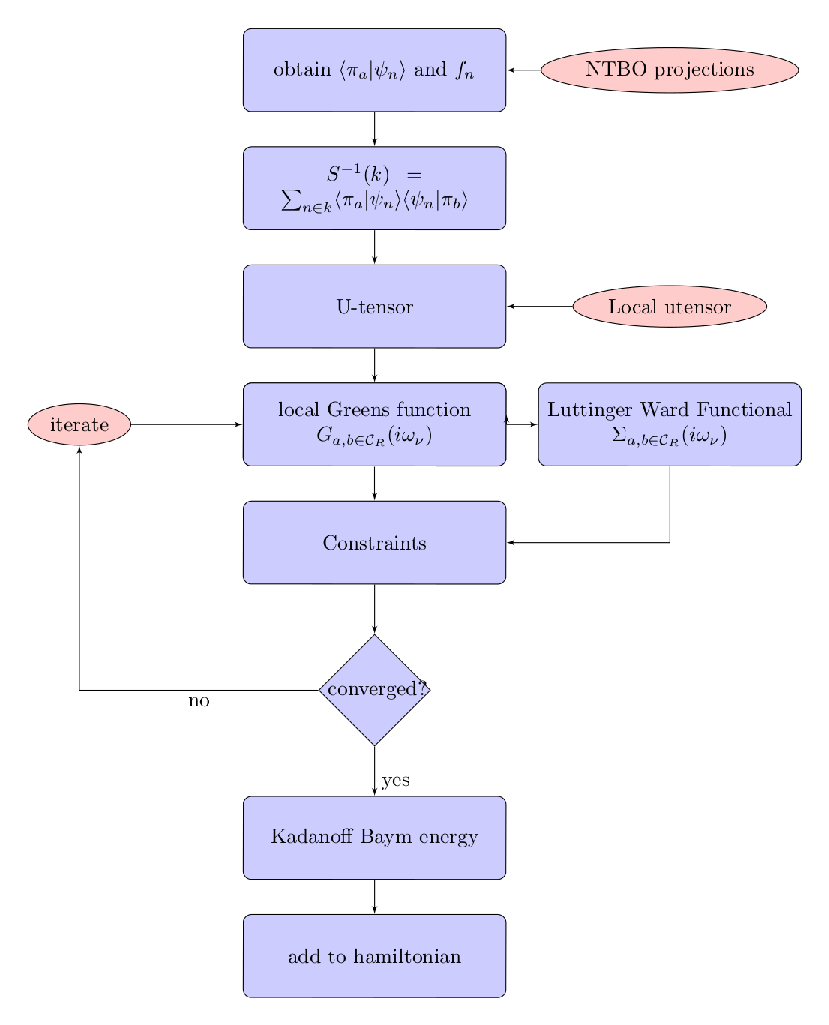
\includegraphics[width=0.5\linewidth]
{Figs/TikZ/FlowdiagramDMFTinterface/flow.eps}
\end{center}

%====================================================================
\subsection{Data exchange of the Object wit the outer world}
%====================================================================


%====================================================================
\subsection{DMFT\$GREEN}
%====================================================================
DMFT\$GREEN is the main subroutine of the DMFT object. It is called
from the LMTO object, which also provides the  projections onto the
tight-binding orbitals.

\begin{verbatim}
call dmft_ini()
call dmft_collecthamiltonian()  
call dmft_collectfulldenmat()  
call dmft_utensor() 
call dmft_smat()
call dmft_natorb()
call dmft_hrho()
call dmft_constraints('hrho')
do iter=1,3
  call dmft_gloc_withatomset() 
  call dmft_solver(etot) 
  call dmft_constraints('h0')
enddo ! end of loop over iterations to enforce constraint
call dmft_detot(svar)
etot=etot+svar      
call energylist$set('dmft interface',etot)
call energylist$add('local correlation',etot)
call energylist$add('total energy',etot)
call dmft_addtohpsi()
\end{verbatim}

\begin{enumerate}
\item \verb|DMFT_COLLECTHAMILTONIAN|: The orbital coefficients
  $\langle\pi_a|\psi_n\rangle$ have been calculated by the LMTO object
  and they are kept in the module of \verb|paw_waves|.
\begin{eqnarray}
\langle\pi_a|\psi_n\rangle&&
\\
\rho_{a,b}(\vec{k})=\sum_n
\langle\pi_a|\psi_n(\vec{k})\rangle f_n(\vec{k})
\langle\psi_n(\vec{k})|\pi_b\rangle
\end{eqnarray}
The orbital coefficients are kept as
\verb|kset(ik)%pipsi(ndim,nchi,nb,nspin)|. The k-dependent density
matrix is kept as \verb|kset(ik)%rho(nchi,nchi,ndimd)|.

\petertt{The name DMFT\_COLLECTHAMILTONIAN is misleading,
  because we only collect the orbital coeffcients and the density
  matrix.}
%
\item \verb|DMFT_COLLECTFULLDENMAT|: Calculates the local density matrix,
  but for all orbitals on each atom. This is needed for the double
  counting term.

 \petertt{This still uses the orbital coefficients and occupations
   from the PAW\_WAVES module, instead of using the orbital
   coefficients or dthe k-dependent density matrix from KSET.}

 \petertt{The name DMFT\_COLLECTFULLDENMAT is misleading.}
%
\item \verb|DMFT_UTENSOR|: (see also
  section~\ref{sec:routinedmftutensor}) The local U-tensor is
  collected from the onsite elements \verb|POTPAR(ISP)%TAILED%U|
  calculated in the \verb|paw_LMTO| object. It is directly converted
  from the ``tailed representation'' into the basis of local orbitals.
\begin{eqnarray}
U_{a,b,c,d}=\alpha\int d^4x\int d^4x'\;
\frac{e^2\chi^*_a(\vec{x})\chi^*_b(\vec{x'})\chi_c(\vec{x})\chi_d(\vec{x'})}
{4\pi\epsilon_0|\vec{r}-\vec{r'}|}
\label{eq:defutensordmftobject}
\end{eqnarray}
Only the U-tensor for equal spin-electrons is stored. $\alpha$ is a
scale factor that mimics the screening of the U-tensor. It is called
\verb|LHFWEIGHT|.

The scaled U-tensor is kept as \verb|ATOMSET(iat)%U|
%
\item \verb|DMFT_SMAT|: The inverse overlap matrix $\mat{S}^{-1}$ is
  calculated as
\begin{eqnarray}
\mat{S}^{-1}(\vec{k})
=\sum_n\langle\pi_a|\psi_n(\vec{k})\rangle\langle\psi_n(\vec{k})|\pi_b\rangle
\end{eqnarray}
Note that the inverse overlap matrix is spin and orbital dependent.
$\mat{S}(\vec{k})$ is pot on the KSET structure as \verb|KSET%SINV| 
and $\mat{S}^{-1}(\vec{k})$ as \verb|KSET%SMAT| 
%
%===============natorb=================================================
\item \verb|DMFT_NATORB|: (see also section~\ref{sec:routinedmftnatorb})
  Construct the eigenstates $|\phi_j\rangle$ of the single site
  density matrix
\begin{eqnarray}
\hat{\rho}_R|\phi_{R,i}\rangle=|\phi_{R,i}\rangle f'_{R,i}
\end{eqnarray}
These states will be called local natural orbitals.

The orbital coefficients of the local natural orbitals are calculated as
\footnote{
\begin{eqnarray}
\underbrace{\sum_{a,b}|\chi_a\rangle\langle\pi_a|\hat{\rho}_R|\pi_b\rangle
\langle\chi_b|}_{\hat{\rho}_R}
\underbrace{\sum_c|\chi_c\rangle x_{c,j}}_{|\phi_{R,j}\rangle}
=\underbrace{\sum_a|\chi_a\rangle x_{a,j}}_{|\phi_{R,j}\rangle} f'_{R,j}
\nonumber\\
\sum_{b,c}\langle\pi_a|\hat{\rho}_R|\pi_b\rangle
\langle\chi_b|\chi_c\rangle x_{c,j}
=x_{a,j}f'_{R,j}
\end{eqnarray}
Now, introduce $y_{a,j}=\sum_b\langle\chi_a|\chi_b\rangle x_{b,j}$
\begin{eqnarray}
\sum_{b}\langle\pi_a|\hat{\rho}_R|\pi_b\rangle y_{b,j}
=\sum_b S^{-1}_{a,b}y_{b,j}f'_{R,j}
\end{eqnarray}
which is a generalized eigenvalue problem for the vectors $\vec{y}_j$,
which are converted into orbital coefficients by multiplication with
$\mat{S}^{-1}$.
\begin{eqnarray}
|\phi_{R,j}\rangle=\sum_{a,b}|\chi_a\rangle S^{-1}_{a,b} y_{b,j}
\end{eqnarray}
The local natural orbitals are orthonormal in the sense
\begin{eqnarray}
\langle\phi_{R,i}|\phi_{R,j}\rangle
=\sum_{a,b,c,d}
y^*_{a,i}S^{-1}_{a,c}
\underbrace{\langle\chi_c|\chi_d\rangle}_{(\mat{S}^{-1})^{-1}}
 S^{-1}_{d,b} y_{b,j}
=\sum_{a,b}y^*_{a,i}S^{-1}_{a,b}y_{b,j}=\delta_{i,j}
\end{eqnarray}
}
\begin{eqnarray}
\sum_{b}\langle\pi_a|\hat{\rho}_R|\pi_b\rangle y_{b,j}
&=&\sum_b S^{-1}_{R,a,b}y_{b,j}f'_{R,j}
\qquad\text{with $\vec{y}^\dagger_i \mat{S}^{-1}_R\vec{y}_{j}=\delta_{i,j}$}
\\
\langle\pi_a|\phi_{R,j}\rangle&=&\sum_{b} S^{-1}_{R,a,b} y_{b,j}
\end{eqnarray}

The local density matrix $\mat{\rho}_R$ andf the local inverse overlap
matrix $\mat{S}^{-1}_R$ are obtained as Brillouin zone intergral
projected onto the lcoal site
\begin{eqnarray}
\mat{\rho}_R&=&\mat{P}_R\Bigl[
\sum_{\vec{k}} w_{\vec{k}}\mat{\rho}(\vec{k})
\Bigr]\mat{P}_R
\nonumber\\
\mat{S}^{-1}_R&=&\mat{P}_R\Bigl[
\sum_{\vec{k}} w_{\vec{k}}\mat{S}^{-1}(\vec{k})
\Bigr]\mat{P}_R
\end{eqnarray}

The transformation matrices are stored in the fully non-collinear data
model in \verb|atomset%natorb%piphi| and the vectors $\vec{y}_j$ are
stored as \verb|atomset%natorb%chiphi|.

\petertt{The vector $y$ is used for the transformation to the local
  natural orbitals in the solver interface. Check if this is
  correct. should it be the vector $x$?}
%
\item \verb|DMFT_HRHO|: For each k-point solve the generalized
  eigenvalue problem
\begin{eqnarray*}
\mat{\rho}(k)\mat{V}(\vec{k})=
\mat{S}^{-1}(\vec{k})\mat{V}(\vec{k})\mat{f}''(\vec{k})
\end{eqnarray*}
where $\mat{f}''(\vec{k})$ is a diagonal matrix that contains
k-dependent occupations. (They differ from the occupations $f_n$ of
the natural orbitals $|\psi_n\rangle$.)
\begin{eqnarray}
\bar{\mat{h}}(\vec{k})-\mu=\mat{V}^{\dagger,-1}(\vec{k})\; k_B
\ln\left[
\frac{\mat{1}-\mat{V}^\dagger(\vec{k})\mat{\rho}(\vec{k})\mat{V}(\vec{k})}
{\mat{V}^\dagger(\vec{k})\mat{\rho}(\vec{k})\mat{V}(\vec{k})}
\right]\mat{V}^{-1}(\vec{k})
\end{eqnarray}
$\bar{\mat{h}}$ is kept as \verb|KSET%HRHO|.
%
\item \verb|DMFT_CONSTRAINTS|: Determines $\mat{h}'(\vec{k})$ such that
\begin{eqnarray}
\mat{\rho}(\vec{k})=k_BT\sum_\nu \Bigl[(i\omega_\nu+\mu)\mat{S}(\vec{k})-
\bar{\mat{h}}+\mat{\Gamma}-\mat{\Sigma}^{\hat{W}_2}_{dyn}(i\omega_\nu)\Bigr]^{-1}
\end{eqnarray}
$\mat{h'}$ is kept as \verb|KSET%H0|.
%
\item \verb|DMFT_GLOC|: The local Green's function is obtained as
  Brillouin zone integral over the k-dependent greens function after
  projecting onto the correlated orbitals on the specified site.
\begin{eqnarray}
\mat{G}_R(i\omega_\nu)=\sum_k w(\vec{k})
\Bigl[(i\omega_\nu+\mu)\mat{S}(\vec{k})-
\bar{\mat{h}}+\mat{\Gamma}-\mat{\Sigma}^{\hat{W}_2}_{dyn}(i\omega_\nu)\Bigr]^{-1}_R
\end{eqnarray}

The result and its Laurent expansion terms are stored in
\verb|atomset%gloc| and \verb|atomset%gloclaur|.
%
\item \verb|DMFT_SOLVER|: Calculates the self energy for the local
  Green's functions. The Hartree-Fock term is separated out and
  calculated directly. Only the dynamic contribution is taken from an
  external solver. The double counting term is calculated as in the
  LMTO module. \textbf{For the double counting in the HF approximation
    only the exchange part is removed, while here also the correlation
    contribution should be taken out, because that is explicitly
    added.}

  The Hartree-Fock contribution is added directly to the double
  counting term. Thus the self energy \verb|atomset%sigma| is only
  the dynamical contribution.

Green's function and U-tensor are transformed into the representation
of orthonormal local orbitals, and the self-energy is transformed back
accordingly.

The external solver shall evaluate
\begin{eqnarray}
\Phi^{LW}[\mat{G}(i\omega_\nu),\hat{W}]
-\Phi^{LW,HF}[\mat{G}(i\omega_\nu),\hat{W}]
\end{eqnarray}
where
\begin{eqnarray}
  \Phi^{LW,HF}[\mat{G},\hat{W}]
  &=&
  \frac{1}{2}
  \frac{1}{\beta^{2}} 
  \sum_{\nu,\nu'} e^{i \beta \hbar \omega_\nu 0^{+}} e^{i \beta \hbar \omega_{\nu'} 0^{+}}
  \sum_{a,b,c,d}
  U_{a,b,d,c} 
  \nonumber\\ 
  &&\hspace{-1.2cm}\times\Big(
  G_{d,a}(i\omega_\nu)G_{c,b}(i\omega_{\nu'})
  -  G_{c,a}(i\omega_\nu)G_{d,b}(i\omega_{\nu'})
  \Big) 
\nonumber\\
&=& \frac{1}{2}
  \sum_{a,b,c,d}
  U_{a,b,d,c} \Bigl(
  \rho_{d,a}\rho_{c,b} -  \rho_{c,a}\rho_{d,b}\Bigr)
  \Big) 
\end{eqnarray}
Correspondingly, the self energy to be returned must have the
Hartree-Fock term subtracted out. That is, the double counting term
must be the Hartree-Fock term.
\begin{eqnarray*}
\Sigma_{a,b}(i\omega_\nu)=\frac{\beta\partial\Phi^{LW}}
{\partial G_{b,a}(i\omega_\nu)}-\sum_{c,d}\Bigl(U_{a,c,b,d}-U_{a,c,d,b}\Bigr)
\rho_{d,c}
\end{eqnarray*}

The external solver may make approximations to the U-tensor or to the
Kadanoff-Baym functional. However, they need to be consistent for
Luttinger-Ward functional and the corresponding Hartree-Fock
term. Thus, it is ensured that there is no approximation made beyond
the dynamic effects.

%
\item \verb|DMFT_DETOT|: Adds the non-local contribution to the total energy
\begin{eqnarray}
&-&\frac{1}{\beta}\sum_\nu\Tr\Bigl\lbrace
\ln\Bigl[
\mat{1}-
\Bigl(i\hbar\omega_\nu+\mu)\mat{1}-\bar{\mat{h}}\Bigr)^{-1}
\Bigl(
\mat{\Sigma}^{\hat{W}_2}_{dyn}(i\omega_\nu)-\mat{\Gamma}\Bigr)
\Bigr]
\nonumber\\&&
+\Bigl(\mat{\Sigma}^{\hat{W}_2}_{dyn}(i\omega_\nu)
-\mat{\Gamma}\Bigr)\mat{G}(i\omega_\nu)
+
\Bigl[
\mat{G}(i\omega_\nu)
-\Bigl(i\hbar\omega_\nu+\mu)\mat{1}-\bar{\mat{h}}\Bigr)^{-1}
\Bigr[
\mat{\Gamma}\Bigr\rbrace
\end{eqnarray}
\begin{itemize}
  \item \textbf{At this point I am still using the Dahlen trick.}  
  \item \textbf{Is it correct that only the dynamic self energy is used?}
\end{itemize}
%
\item \verb|DMFT_ADDTOHPSI|: Adds the energy derivative to
  \verb|this%htbc| of the \verb|waves_module|. There are two
  contributions, a k-dependent term which is restricted to the
  correlated orbitals and an site-dependent term that acts on all
  local orbitals.
\begin{itemize}
\item The site-specific term contains the double counting term for the
  DFT functional and the Hartree-Fock contribution to the self energy.
\end{itemize}
\end{enumerate}



%====================================================================
\subsection{DMFT\_INI}
%====================================================================

%====================================================================
\subsubsection{Hardwired data}
%====================================================================
\begin{itemize}
\item NOMEGA ($N_\omega$)
\end{itemize}

%====================================================================
\subsubsection{Inherited data}
%====================================================================
\begin{itemize}
\item NDIM from \verb|waves_module|
\item NSPIN from \verb|waves_module|
\item NKPTL from \verb|waves_module|
\item NAT  from \verb|ATOMLIST| Object
\item isp(IAT)
\item WKPT and (NKPT,KMAP) from \verb|DYNOCC| Object
\item KBT from \verb|dynocc$getr8a('temp')| from
  \verb|paw_occupations.f90|
\item \verb|atomset(iat)%lhfweight| from \verb|lmto_module|
\end{itemize}

%====================================================================
\subsubsection{Derived data}
%====================================================================
\begin{itemize}
\item NDIMD (=1 for NDIM=1,NSPIN=1; =2 for NDIM=1,NSPIN=2; =4 for
  NDIM=2,NSPIN=1)
\item List of positive Matsubara frequencies
\begin{eqnarray}
\omega_\nu=(2\nu-1)\pi k_BT \qquad\text{for $\nu=1,\ldots,N_\omega$}
\end{eqnarray}
\item Atomset structure
\begin{center}
 \begin{tabular}{ll}
 \verb|atomset\%nloc| & number of correlated orbits on this atom \\
\verb|atomset\%ICHI1| & first value of ICHI index for this atom\\
\verb|atomset\%ICHI2| & last value of ICHI index for this atom\\
\end{tabular}
\end{center}
%
\item KSET structure
\begin{center}
 \begin{tabular}{ll}
 \verb|KSET\%WKPT| & geometric k-point weight\\
\end{tabular}
\end{center}
\end{itemize}

%====================================================================
\subsection{DMFT\_UTENSOR}
\label{sec:routinedmftutensor}
%====================================================================
Obtain the onsite Utensor for all local orbitals from subroutine
\verb|dmft_ulocal| reduces it to the entries for the correlated
orbitals.

In \verb|DMFT_ULOCAL| it obtains the local U-tensor from the
\verb|POTPAR%TAILED%U| and \verb|SBAR| of the LMTO Object. This object
contains the extended $\phi$ and $\dot{\phi}$ functions
\begin{eqnarray}
|\chi_a\rangle=|\phi_a\rangle-
\sum_{b; R_b=R_a}|\dot{\bar{\phi}}_b\rangle \bar{S}_{a,b}
\end{eqnarray}


The U-tensor is constructed in \verb|LMTO\_MAKETAILEDPARTIALWAVES|.
\verb|LMTO\_ULITTLE| constructs
\begin{eqnarray}
u_{\ell,a,b,c,d}
=\frac{2\ell+1}{4\pi}
\int dr\; r^2R_c(r)R_d(r)\Bigl[\int d^3r'\;V_\ell(r,r')R_a(r')R_b(r')\Bigr]
\end{eqnarray}
where the kernel $V_\ell(r,r')$ is the one used by $RADIAL\$POISSON$.
\textbf{There is a input parameter that determines which $\ell$ values are
considered.}

In \verb|LMTO_UTENSOR| the U-tensor elements are composed according to
\begin{eqnarray}
U_{a,b,c,d}=\sum_{ell}\frac{4\pi}{2\ell+1}\sum_{m=-\ell}^\ell
u_{\ell,b,d,c,a} C_{L,L_b,L_d}C_{L,L_c,L_a}
\end{eqnarray}

The U-tensor is screened by a factor \verb|LHFWEIGHT|. It is obtained
from the \verb|lmto_module| either as the global value \verb|HFWEIGHT|
or the individual value from hybridsetting. This very same factor is
used for the double counting term.

Thus the U-tensor is defined as\footnote{$\vec{x}=(\vec{r},\sigma)$}
in Eq.~\ref{eq:defutensordmftobject}, i.e. as
\begin{eqnarray}
U_{a,b,c,d}=\int d^4x\int d^4x'\;
\frac{e^2\chi^*_a(\vec{x})\chi^*_b(\vec{x'})\chi_c(\vec{x})\chi_d(\vec{x'})}
{4\pi\epsilon_0|\vec{r}-\vec{r'}|}
\end{eqnarray}
The U-tensor contributes only if $\sigma_a=\sigma_c$ and if
$\sigma_b=\sigma_d$.
With this definition the Hartree and exchange  energy have the form
\begin{eqnarray}
E_H=\frac{1}{2}\sum_{a,b,c,d}U_{a,b,c,d}\;\rho_{c,a}\rho_{d,b}
\nonumber\\
E_X=\frac{1}{2}\sum_{a,b,c,d}U_{a,b,c,d}\;\rho_{c,b}\rho_{d,a}
\end{eqnarray}


%====================================================================
\subsection{DMFT\_NATORB}
\label{sec:routinedmftnatorb}
%====================================================================
Construct natural orbitals in the space of correlated orbitals on one
site.

For this purpose, I redefine the unity operator for the sub Hilbert
space of correlated orbitals.
\begin{eqnarray}
\hat{1}_{\mathcal{C}_R}
=\sum_{\alpha,\beta}\sum_n
|\chi_\alpha\rangle
\langle\pi_\alpha|\psi_n\rangle\langle\psi_n|\pi_\beta\rangle
\langle\chi_\beta|
\end{eqnarray}
which allows one to identify the inverse overlap matrix in this sub-Hilbert space.
\begin{eqnarray}
\mat{S}^{-1}_{\alpha,\beta}
=\sum_{\alpha,\beta}\sum_n
\langle\pi_\alpha|\psi_n\rangle\langle\psi_n|\pi_\beta\rangle
\end{eqnarray}
Note,however, that this matrix lives only on a single site! We can
obtain it from the k-dependent $\mat{S}^{-1}$ by summing over k-points
and cutting out the corresponding submatrix. However, it is not
allowed to do the same thing for the overlap matrix itself!

The one-particle density matrix in this sub-Hilbert space has the form
\begin{eqnarray}
\hat{\rho}_{\mathcal{C}_R}
=\sum_{\alpha,\beta}\sum_n
|\chi_\alpha\rangle
\langle\pi_\alpha|\psi_n\rangle f_n \langle\psi_n|\pi_\beta\rangle
\langle\chi_\beta|
\end{eqnarray}

The eigenvalue equation
\begin{eqnarray}
\hat{\rho}|\phi_n\rangle=|\phi_n\rangle f_n
\nonumber\\
\sum_{\alpha,\beta}|\chi_\alpha\rangle
\langle\pi_\alpha|\hat{\rho}|\pi_\beta\rangle\langle\chi_\beta|\phi_j\rangle
=\sum_{\alpha,\beta}|\chi_\alpha\rangle\langle\pi_\alpha|\pi_\beta\rangle
\langle\chi_\beta|\phi_j\rangle f_j
=\sum_{\alpha,\beta}|\chi_\alpha\rangle
\mat{S}^{-1}_{\alpha,\beta}\langle\chi_\beta|\phi_j\rangle \bar{f}_j
\end{eqnarray}
provides us with a new set of occupations $\bar{f}$ of local natural
orbitals and eigenvectors
$\langle\chi_\beta|\phi_j\rangle=V_{\beta,j}$.
\begin{eqnarray}
\mat{\rho}\mat{V}=\mat{S}^{-1}\mat{V}\bar{f}
\qquad\text{with}\qquad
\mat{V}^\dagger\mat{S}^{-1}\mat{V}=\mat{1}
\end{eqnarray}

The natural orbitals are
\begin{eqnarray}
|\phi_j\rangle=\sum_{\alpha,\beta\in\mathcal{C}_R}
\underbrace{|\chi_\alpha\rangle
\mat{S}^{-1}_{\alpha,\beta}\langle\chi_\beta|}_{\mat{1}_{\mathcal{C}_R}}
\phi_j\rangle
=\sum_{\alpha\in\mathcal{C}_R}|\chi_\alpha\rangle
\underbrace{\Bigl(\mat{S}^{-1}\mat{V}\Bigr)_{\alpha,j}}_{\mat{V}^{\dagger,-1}_{\alpha,j}}
\end{eqnarray}

The matrix $\mat{V}$ is placed into the structure
\verb|atomset%natorb%chiphi|, together with the occupations $\bar{f}$
which are in \verb|atomset%natorb%f|. In addition we store
$\mat{S}^{-1}\mat{V}=\mat{V}^{\dagger,-1}$ in
\verb|atomset%natorb%piphi| All data in \verb|atomset%natorb| are
stored in the fully non-collinear model.

%====================================================================
\subsection{DMFT\_HRHO}
%====================================================================
The conversion of occupations into energies is done in the routine
\verb|DMFT_EOFF|.
\begin{eqnarray}
\epsilon=k_B
\begin{cases}
\ln\left(\frac{1-f}{f}\right) &\text{for $f_0<f<1-f_0$}\\
a+b(f-f_0)&\text{for $f<f_0$}\\
-a+b(f-(1-f_0))&\text{for $f>1-f_0$}\\
\end{cases}
\end{eqnarray}
where $a$ and $b$ are determined such that the mapping is
differentiable. The value of $f_0$ is currently set to $10^{-6}$.

%====================================================================
\subsection{DMFT\_CONSTRAINTS}
\label{sec:routinedmftconstraints}
%====================================================================
%====================================================================
\subsubsection{Green's function}
%====================================================================
The Green's function is calculated as follows
\begin{eqnarray}
\mat{G}(\vec{k},i\omega_\nu)&=&
\Bigl[
(i\omega_\nu+\mu)\mat{S}(\vec{k})-\bar{\mat{h}}(\vec{k})+\mat{\Gamma}(\vec{k})
-\sum_R\mat{\Sigma}^{dyn}_R(i\omega_\nu)
\Bigr]^{-1}
\end{eqnarray}
As described in section~\ref{sec:laurentgreen} on
p.~\pageref{sec:laurentgreen}, the Laurent-expansion coefficients are
\begin{eqnarray}
\mat{G}^{(1)}(\vec{k})&=&\mat{S}^{-1}(\vec{k})
\nonumber\\
\mat{G}^{(2)}(\vec{k})&=&\mat{S}^{-1}(\vec{k})
\Bigl(-\mu\mat{S}(\vec{k})+\bar{\mat{h}}(\vec{k})-\mat{\Gamma}(\vec{k})
+\mat{\mathcal{S}}^{(1)}_{dyn}(\vec{k})
\Bigr)
\mat{S}^{-1}(\vec{k})
\nonumber\\
\mat{G}^{(3)}(\vec{k})&=&
\mat{S}^{-1}(\vec{k})
\biggl[
\mat{\mathcal{S}}^{(2)}_{dyn}(\vec{k})+
\Bigl(-\mu\mat{S}(\vec{k})+\bar{\mat{h}}(\vec{k})-\mat{\Gamma}(\vec{k})
+\mat{\mathcal{S}}^{(1)}_{dyn}(\vec{k})\Bigr)
\nonumber\\
&&\times\mat{S}^{-1}(\vec{k})
\Bigl(-\mu\mat{S}(\vec{k})+\bar{\mat{h}}(\vec{k})-\mat{\Gamma}(\vec{k})
+\mat{\mathcal{S}}^{(1)}_{dyn}(\vec{k})\Bigr)
\biggr]
\mat{S}^{-1}(\vec{k})
\nonumber\\
\end{eqnarray}

%============================================================================
\subsubsection{Update $\mat{\Gamma}$}
%============================================================================
\begin{myshadowminipage}{Update $\Gamma$}
The following two equations are solved iteratively
\begin{eqnarray}
\delta\mat{\rho}(\vec{k})&=&
\biggl(\frac{1}{\beta}\sum_\nu
\underbrace{\Bigl[
(i\omega_\nu+\mu)\mat{S}(\vec{k})-\bar{\mat{h}}(\vec{k})+\mat{\Gamma}(\vec{k})
-\sum_R\mat{\Sigma}^{dyn}_R(i\omega_\nu)
\Bigr]^{-1}}_{\mat{G}(\vec{k})}\biggr)-\mat{\rho}(\vec{k})
\nonumber\\
\mat{\Gamma}(\vec{k})&=&\mat{\Gamma}(\vec{k})-\frac{4}{\beta}\mat{S}(\vec{k})
\delta{\rho}(\vec{k})
\mat{S}(\vec{k})
\end{eqnarray}
until $\delta\mat{\rho}$ vanishes.
\end{myshadowminipage}

This equation is a Newton scheme with the Green's function in the
slope estimate replaced by the non-interacting Green's function with
zero potential self energy and chemical potential. 


\begin{eqnarray}
\delta\mat{\rho}(\mat{\Gamma})=\delta\mat{\rho}(\mat{\Gamma}_0)
-\frac{1}{\beta}\sum_\nu \mat{G}(\mat{\Gamma}-\mat{\Gamma}_0)\mat{G}+...
\end{eqnarray}
Now we approximate $\mat{G}$ by $(i\hbar\omega_\nu)^{-1}\mat{S}^{-1}$
\begin{eqnarray}
\delta\mat{\rho}(\mat{\Gamma})&=&\delta\mat{\rho}(\mat{\Gamma}_0)
-
\underbrace{\frac{1}{\beta}
\Bigl[\sum_\nu\frac{1}{(i\hbar\omega_\nu)^2} \Bigr]}
_{-\beta/4}
\mat{S}^{-1}(\mat{\Gamma}-\mat{\Gamma})\mat{S}^{-1}+...
\nonumber\\
\Rightarrow\qquad\mat{\Gamma}&=&\mat{\Gamma}_0
+\frac{4}{\beta}
\mat{S}
\Bigl(\underbrace{\delta\mat{\rho}(\mat{\Gamma})}_{=0}-\delta\mat{\rho}(\mat{\Gamma}_0)\Bigr)
\mat{S}
\end{eqnarray}


\petertt{Should
  there be convergence problems, it may be improved by using the
  static Green's function $\mat{G}_\rho$ instead.}




%====================================================================
\subsection{DMFT\_SOLVER}
%====================================================================
The solver first calculates the Hartree-Fock contribution to the
Luttinger-Ward functional as defined in Eq.~\ref{eq:philwhf} and the
corresponding self energy. Because the Hartree-Fock self energy is
static and because it does not affect the density matrix constraint,
it is added together with the double counting correction to
\verb|atomset%denmat%h|.


Then the double counting correction is calculated. \textbf{At the
  moment we still subtract out only the exchange part, which is
  consistent with the hybrid functionals but not as double counting
  for correlation.}

Finally the data are prepared for the solver in
\verb|DMFT_dynamicsolver|. The dynamicsolver transforms all data into
a spin-orbital representation of orthonormal states, which may be
either natural orbitals derived from the local density matrix or which
may be eigenstates of the local overlap matrix.

%====================================================================
%\section{Helper routines}
%====================================================================

\appendix
%====================================================================
%\chapter{Helper routines}
%====================================================================
%====================================================================
\chapter{Matsubara frequencies}
\label{app:matsubarafreq}
%====================================================================

The Matsubara frequencies for Fermions are
\begin{eqnarray*}
\omega_\nu=(2\nu+1)\frac{\pi}{\hbar\beta}
\end{eqnarray*}

A Matsubara sum has the general form
\begin{eqnarray*}
\frac{1}{\beta}\sum_{\nu\in z} g(i\omega_\nu)
\end{eqnarray*}
where $g(i\omega_\nu)$ is a analytic function.

%====================================================================
\section{Evaluation using residual theorem}
%====================================================================
In order to evaluate the Matsubara sum we introduce a
\textbf{Matsubara weighting functions}\index{ Matsubara weighting
  functions}, that has simple poles at $i\omega_\nu$, so that we can
exploit the residuum theorem. For Fermions, two such weighting
functions are used
\begin{eqnarray}
h^\pm(z)=\frac{\mp\beta\hbar}{1+\e{\pm\beta\hbar z}}
\end{eqnarray}

The poles of the Matsubara weighting functions obey
\begin{eqnarray}
1+\e{\pm\beta\hbar z}=0
\label{eq:matsubarapolecond}
\end{eqnarray}
With the help of
\begin{eqnarray*}
\e{\pm\beta\hbar z}
=\e{\pm\beta\hbar\Re(z)}\e{\pm i\beta\hbar\Im(z)}
=\e{\beta\hbar\Re(z)}\cos(\beta\hbar\Im(z))
\pm i\e{\beta\hbar\Re(z)}\sin(\beta\hbar\Im(z))
\end{eqnarray*}
\eq{eq:matsubarapolecond} can be rewrfitten in the form
\begin{eqnarray}
\Rightarrow
\e{\pm \beta\hbar\Re(z)}\cos(\beta\hbar\Im(z))=-1
\qquad\text{and}\qquad
\e{\pm \beta\hbar\Re(z)}\sin(\beta\hbar\Im(z))=0
\end{eqnarray}
The second equation is obeyed for
\begin{eqnarray}
\Im(z)=\frac{n\pi}{\hbar\beta}\qquad\text{for arbitrary integer $n$}
\end{eqnarray}
The first equation yields
\begin{eqnarray}
-1&=&\e{\pm\beta\hbar\Re(z)}\cos(\beta\hbar\Im(z))
=\e{\pm\beta\hbar\Re(z)}\cos(n\pi)
=\e{\pm\beta\hbar\Re(z)}(-1)^n
\nonumber\\
\Rightarrow
n-1&=&2\nu \qquad\text{for arbitrary integer $\nu$, and $Re(z)=0$}
\nonumber\\
\Rightarrow
n&=&2\nu+1
\end{eqnarray}
Thus we obtain that the poles of the Matsubara weighting function lie
at the Matsubara frequencies.
\begin{eqnarray}
z_\nu=i(2\nu+1)\frac{\pi}{\hbar\beta}=i\omega_\nu
\end{eqnarray}

Next we need to show that the weighting function at the poles behaves
like $\frac{1}{z-z_0}+O(|z-z_0|^2)$, where $x_0$ is the position of the pole.
For this purpose we expand the inverse
\begin{eqnarray}
\frac{1}{\mp\hbar\beta}(1+\e{\pm\hbar\beta z})
&=&\frac{1}{\mp\hbar\beta}
(\underbrace{1+\e{\pm\hbar\beta z_0}}_{=0} 
\pm\hbar\beta\underbrace{\e{\pm\hbar\beta z_0}}_{-1}(z-z_0)+O(|z-z_0|^2) )
\\
&=&(z-z_0)+O(|z-z_0|^2) 
\end{eqnarray}



With the help of the Matsubara weighting function we can evaluate the
Matsubara sum as\footnote{Cauchy's Integral formula:
\begin{eqnarray*}
Res(f,z_0)=\frac{1}{2\pi i}\oint_\gamma dz\; f(z)
\end{eqnarray*}
where $\gamma$ is a counter-clockwise countour around a pole $z_0$ of
a function $f$, that can be expanded into a Laurent series about
$z_0$. The Residuum is the prefactor of the term $1/(z-z_0)$ in the
Laurent expansion.}
\begin{eqnarray}
\frac{1}{\beta}\sum_{nu\in Z}g(i\omega_\nu)&=&
\frac{1}{2\pi i\beta}\oint g(z) h^{\pm}(z)
=-\frac{1}{\beta}\sum_{z_0\in\text{poles of g}}
\text{Res}(gh^{\pm},z_0)
\end{eqnarray}





The minus sign occurs because the c ounter clockwise integration of
the contur in the half plane turns into a clock-wise integration about
the pole.

\begin{center}
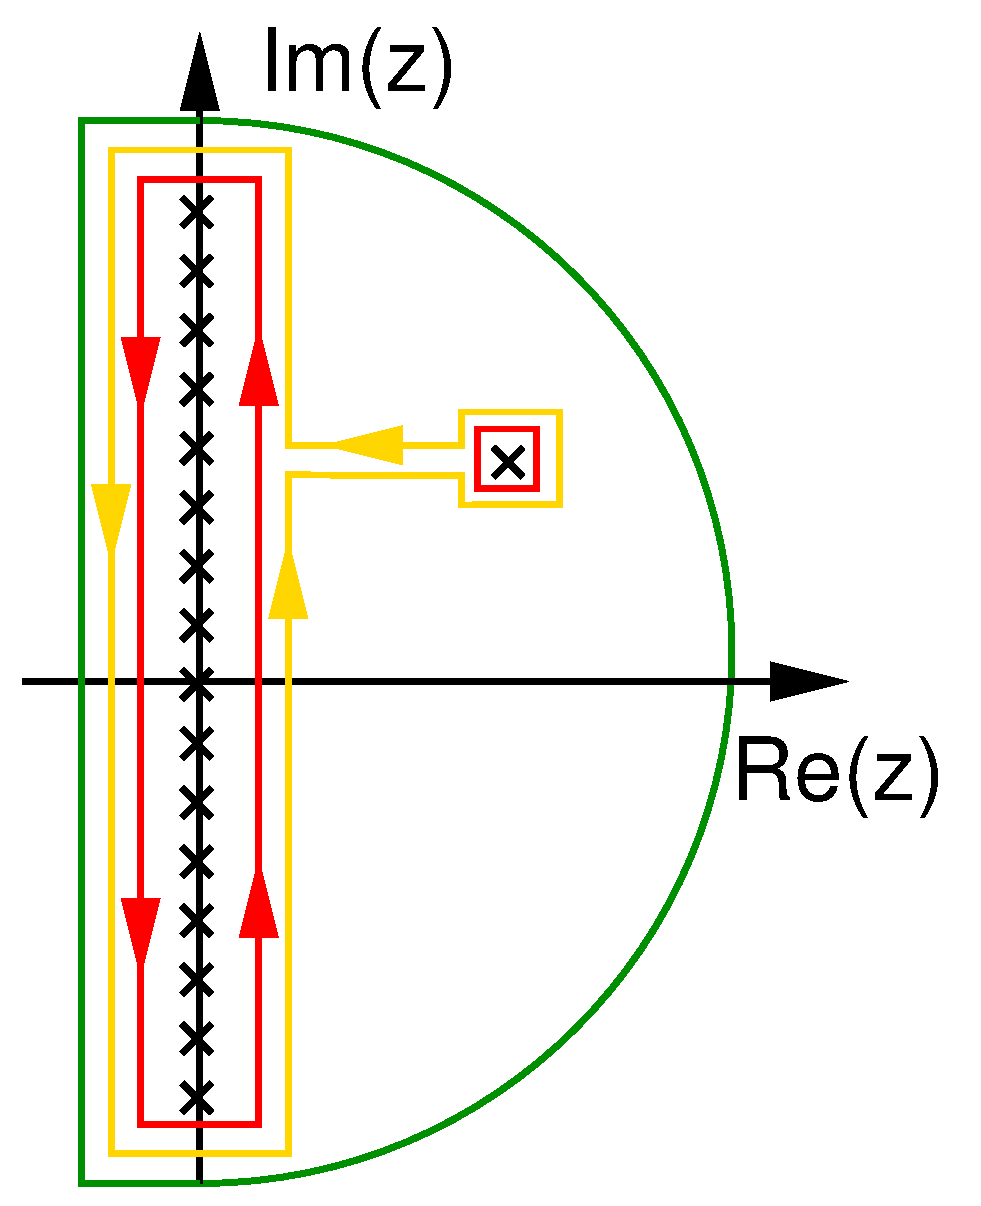
\includegraphics[width=0.25\linewidth]{Figs/Xfig/Matsubaracontour/contour.eps}
\end{center}

The integration is closed in the half plane with $\pm Re(z)>0$, because
we there the corresponding weighting function $h^{\pm}$ decays
exponentially for $Re(z)\rightarrow\pm\infty$.


%====================================================================
\subsection{Matsubara sums}
%====================================================================
From \url{http://en.wikipedia.org/wiki/Matsubara_frequency} we obtain
the following expression for the \textbf{fermionic} summations.  In
these expressions the Matsubara frequencies are\footnote{They differ
  from those of the source by a factor $1/\hbar$.}
\begin{eqnarray}
\omega_\nu=(2\nu+1)\pi/(\hbar\beta)
\end{eqnarray}


\begin{eqnarray}
-k_BT\sum_\nu\ln[-i\hbar\omega_\nu+\epsilon]\e{i\omega_\nu0^+}
&=&-k_BT\ln[1+e^{-\beta \epsilon}]
\\
k_BT\sum_\nu \frac{1}{(i\hbar\omega_\nu-\epsilon)}\e{i\omega_\nu 0^+}
&=&(1+\e{\beta \epsilon})^{-1}
\\
k_BT\sum_\nu \frac{1}{(i\hbar\omega_\nu-\epsilon)^n}
&=&\frac{1}{(k_BT)^{n-1}(n-1)!}
\left.\partial_\epsilon^{n-1}\right|_{x=\beta\epsilon}(1+\e{x})^{-1}
\end{eqnarray}
\begin{center}
\begin{tabular}{|c|c|c|c|c|c|c|c|c|c|c|}
\hline
$j$& 1 & 2 & 3 & 4 & 5 &6 &7 &8 & 9 & 10\\
\hline
$\partial^{j-1}_x(1+\e{x})^{-1}$
&$\frac{1}{2}$ 
&$-\frac{1}{4}$ 
&$0$ 
&$+\frac{1}{8}$ 
&$0$ 
&$-\frac{1}{4}$ 
&$0$ 
&$\frac{17}{16}$
&$0$ 
&$-\frac{31}{4}$
\\
\hline
$\partial^{j-1}_x(1+\e{x})^{-1}$
&$0.5$ 
&$-0.25$ 
&$0$ 
&$+0.125$ 
&$0$ 
&$-0.25$ 
&$0$ 
&$+1.0625$
&$0$ 
&$-7.75$
\\
\hline
\hline
$j$& 11 & 12 & 13 & 14 & 15 &16 &17 &18 & 19 & 20\\
\hline
$\partial^{j-1}_x(1+\e{x})^{-1}$
&$0$ 
&$\frac{691}{8}$ 
&$0$ 
&$-\frac{5461}{4}$ 
&$0$ 
&$\frac{929569}{32}$ 
&$0$ 
&$-\frac{3202291}{4}$
&$0$ 
&$+\frac{221930581}{8}$
\\
\hline
$\partial^{j-1}_x(1+\e{x})^{-1}$
&$0$ 
&$86.375$ 
&$0$ 
&$-1365.25$ 
&$0$ 
&$29.0\times10^3$ 
&$0$ 
&$-800\times10^3$
&$0$ 
&$27.7\times 10^6$ %$+27741322.625$
\\
\hline
\end{tabular}
\end{center}

\begin{figure}[h!]
\begin{center}
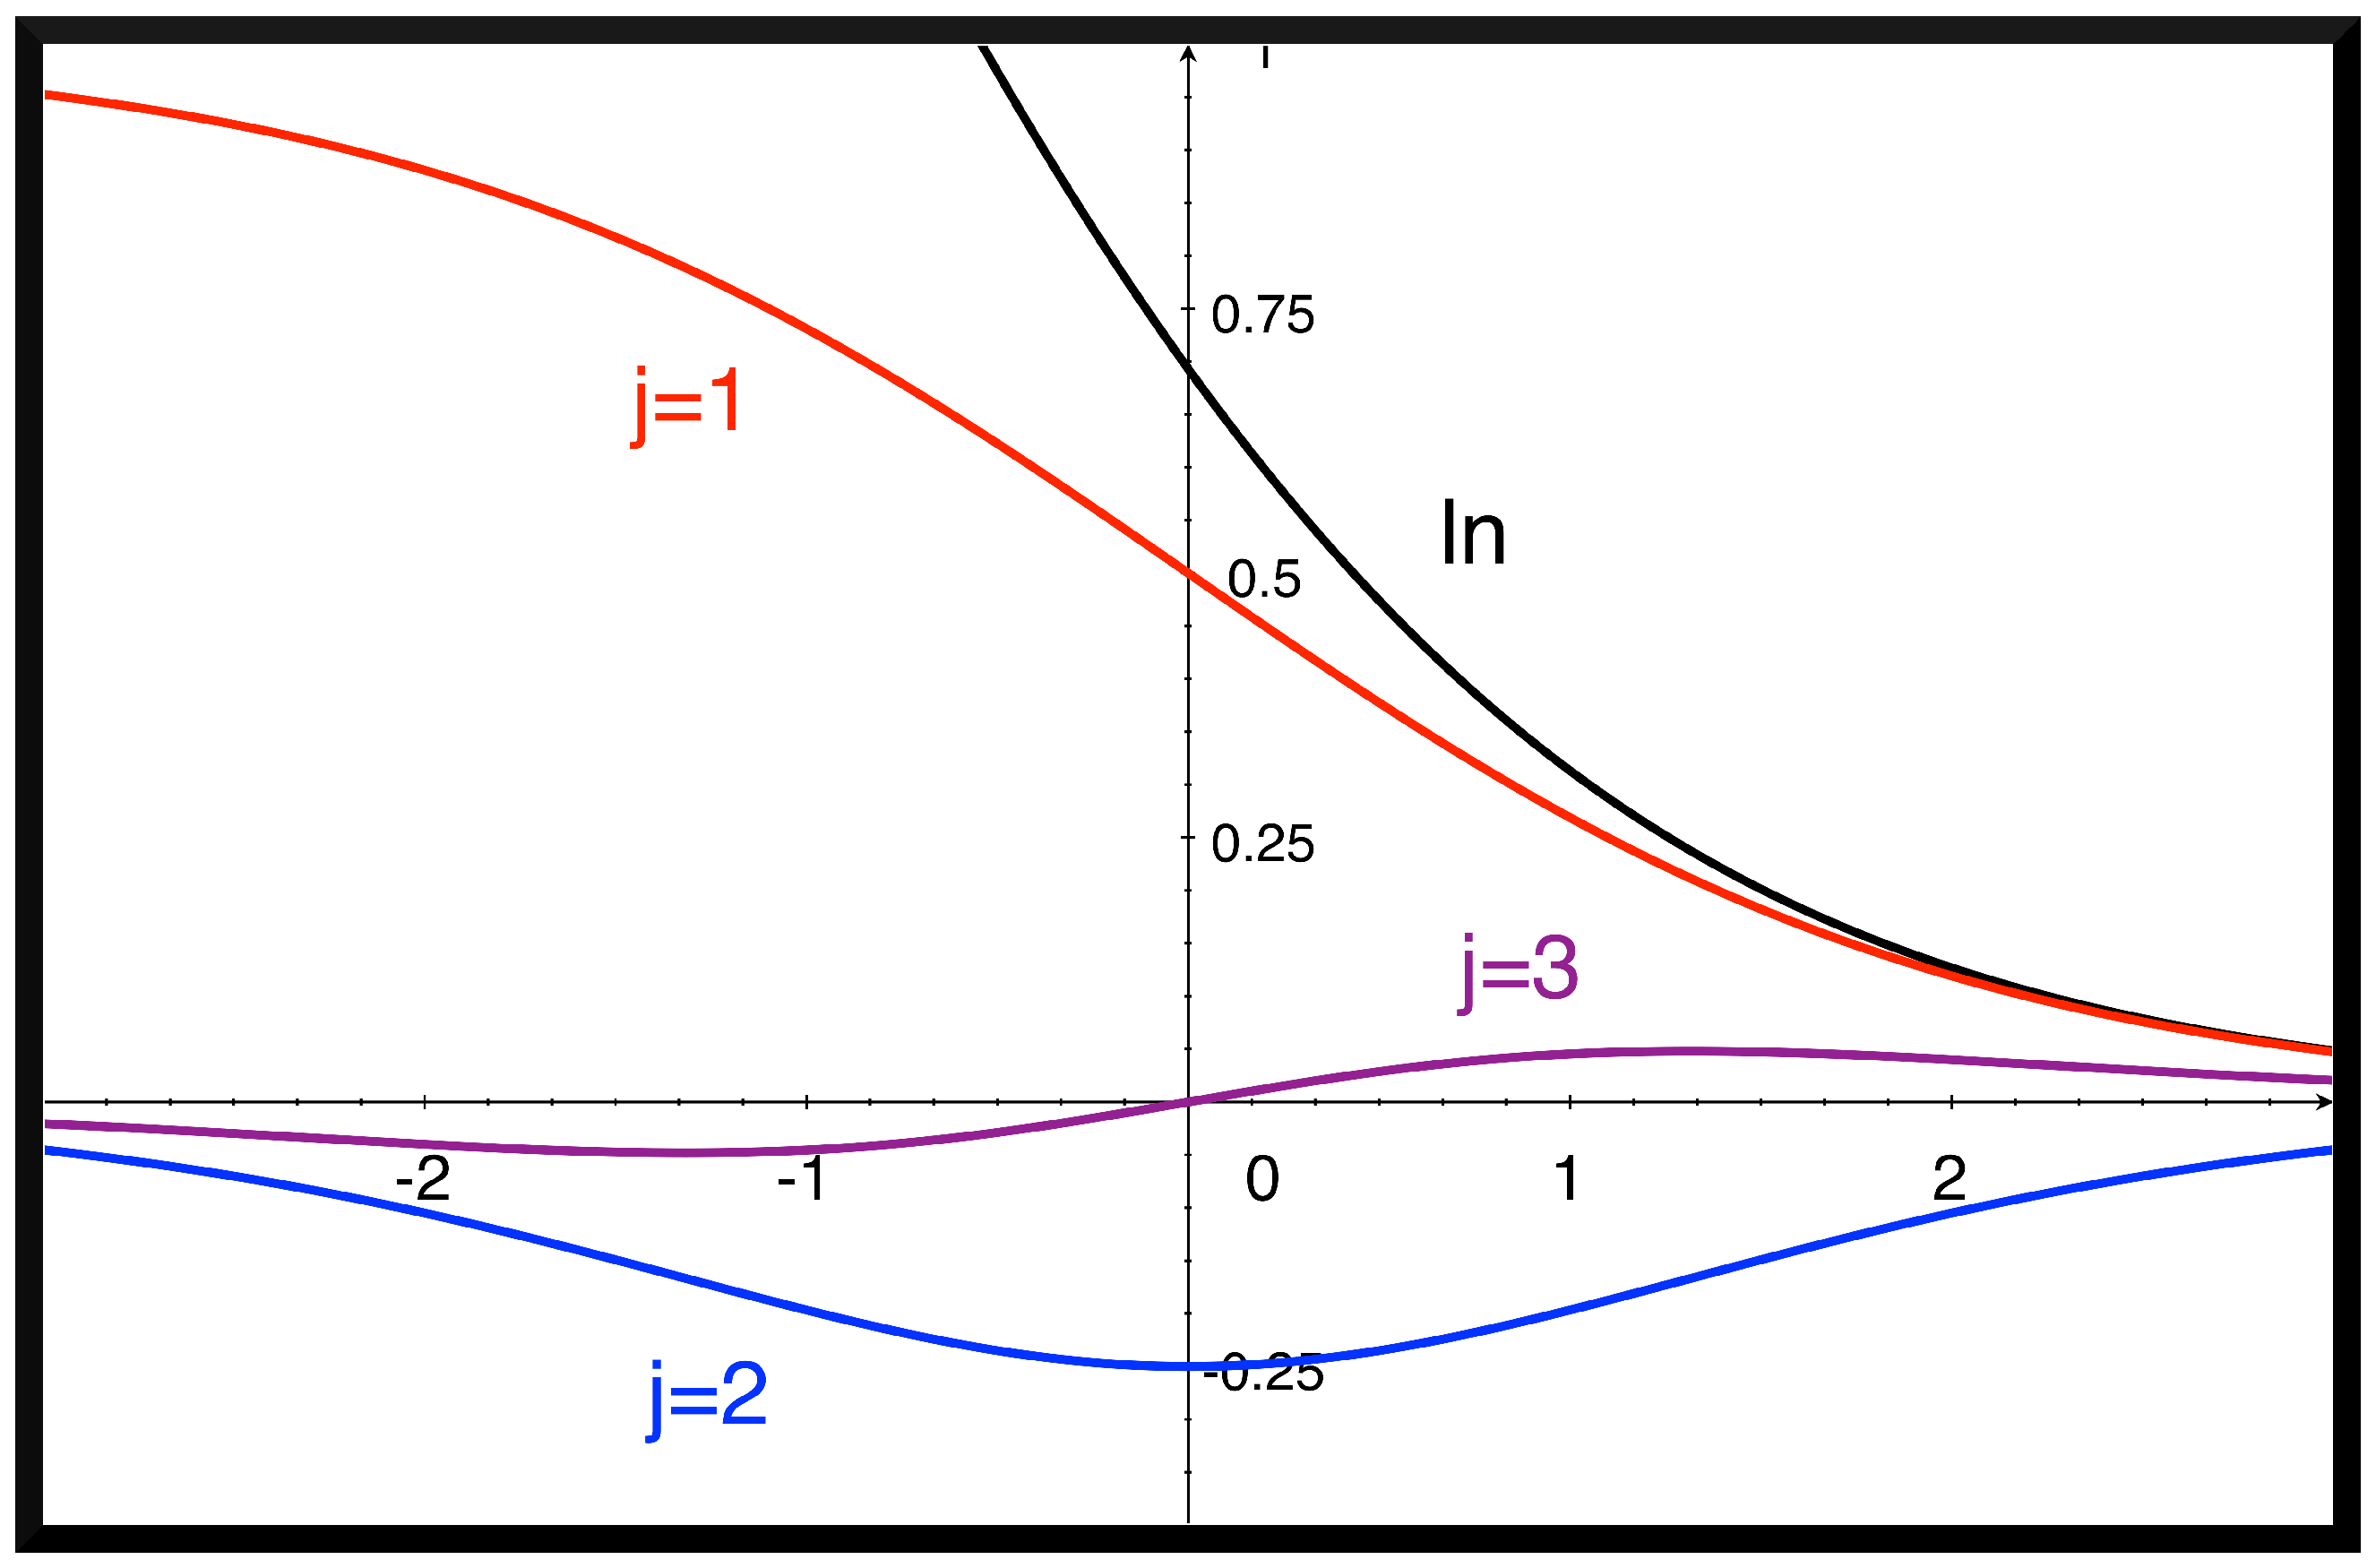
\includegraphics[width=0.8\linewidth,clip=true]
{Figs/Matsubarasums/matsubarasums1.eps}
\end{center}
\caption{\label{fig:matsubarasums} The result of Matsubara sums
  $-k_BT\sum_\nu\ln[-i\hbar\omega_\nu+\epsilon]$, $k_BT\sum_\nu
  \frac{1}{(i\hbar\omega_\nu-\epsilon)}\e{i\omega_\nu 0^+}$,
$k_BT\sum_\nu \frac{1}{(i\hbar\omega_\nu-\epsilon)^2}$ as
  function of energy $\epsilon$.}
\end{figure}



%====================================================================
\subsection{Matsubara sums on finite grids}
%====================================================================
The finite Matsubara sums result in a Fermi function that does not
reach zero or one. In particular, in the limit of e level, that lies
far from the chemical potential, the finite Matsubara sum falls off to
$\frac{1}{2}$.

\begin{figure}[h!]
\begin{center}
\includegraphics[width=0.4\linewidth,clip=true]
{Figs/Xmgrace/FiniteMatsubara/gsumlow.eps}
\includegraphics[width=0.4\linewidth,clip=true]
{Figs/Xmgrace/FiniteMatsubara/gsumhigh.eps}
\end{center}
\caption{\label{fig:finfitematsubara} Fermi function calculated from a
  finite Matsubara sum. The function is shifted by $-\frac{1}{2}$
  because no relgularization has been done. The sums have been
  performed with $2^n$ grid points with $n=0,\ldots,12$ for $k_BT=1.$}
\end{figure}



%====================================================================
\chapter{The Green function}
%====================================================================
We construct the \textbf{lattice Green's function} defined as
\begin{eqnarray}
\hat{G}^{lat}(i\omega_\nu)&=&
\biggl[(i\hbar\omega_\nu+\mu)\hat{1}
-\hat{h}-\Delta\hat{\Sigma}(i\omega_\nu)\biggr]^{-1}
\nonumber\\
&\approx&\sum_{n,n'}|\psi_n\rangle
\underbrace{
\biggl[\langle\psi_{n'}|(i\hbar\omega_\nu+\mu)\hat{1}-\hat{h}
-\Delta\hat{\Sigma}(i\omega_\nu)|\psi_n\rangle\biggr]_{n,n'}^{-1}
}_{G^{lat}_{n,n'}}
\langle\psi_{n'}|
\label{eq:latgreenfunc}
\end{eqnarray}
This expression is approximate, if the set of band states is not
complete. In practice, corrections are required.

In the representation of the band states, the lattice Green's function
has the form
\begin{eqnarray}
G^{lat}_{n,n'}(i\omega_\nu)&=&
\biggl[\langle\psi_{n'}|(i\hbar\omega_\nu+\mu)\hat{1}-\hat{h}
-\Delta\hat{\Sigma}(i\omega_\nu)|\psi_n\rangle\biggr]_{n,n'}^{-1}
\label{eq:latgreenfuncmat}
\end{eqnarray}
Note, that the matrix to be inverted is not necessarily hermitean!

%====================================================================
\section{Generic properties}
%====================================================================
%====================================================================
\subsection{Green's function with negative Matsubara frequencies}
%====================================================================
Green's functions and self energies obey the relation
\begin{eqnarray*}
\mat{G}(-i\omega_\nu)=\mat{G}^\dagger(i\omega)
\end{eqnarray*}
This allows one to store only half of the Green's functions.

Proof:

\begin{eqnarray}
G_{\alpha,\beta}(i\omega_n)&=&
-\frac{1}{\hbar}\int_0^{\hbar\beta} d\tau\;\e{i\omega_n\tau}
\Bigl\langle\mathcal{T}\hat{c}_\alpha(\tau)\hat{c}^\dagger_\beta(0)\Bigr\rangle
\\
\Rightarrow
G_{\alpha,\beta}(-i\omega_n)
&=&
-\frac{1}{\hbar}\int_0^{\hbar\beta} d\tau\;\e{-i\omega_n\tau}
\Bigl\langle\mathcal{T}\hat{c}_\alpha(\tau)\hat{c}^\dagger_\beta(0)\Bigr\rangle
\nonumber\\
&=&
\biggl\lbrace
-\frac{1}{\hbar}\int_0^{\hbar\beta} d\tau\;\e{i\omega_n\tau}
\Bigl\langle\biggl(\e{\beta(\hat{H}-\mu\hat{N})}\hat{c}_\alpha
\e{-\beta(\hat{H}-\mu\hat{N})}\hat{c}^\dagger_\beta\biggr)^\dagger
\Bigr\rangle
\biggr\rbrace^*
\nonumber\\
&=&
\biggl\lbrace
-\frac{1}{\hbar}\int_0^{\hbar\beta} d\tau\;\e{i\omega_n\tau}
\Bigl\langle
\hat{c}_\beta\e{-\beta(\hat{H}-\mu\hat{N})}\hat{c}^\dagger_\alpha
\e{\beta(\hat{H}-\mu\hat{N})}
\Bigr\rangle
\biggr\rbrace^*
\nonumber\\
&\stackrel{cycl. perm}{=}&
\biggl\lbrace
-\frac{1}{\hbar}\int_0^{\hbar\beta} d\tau\;\e{i\omega_n\tau}
\Bigl\langle
\e{\beta(\hat{H}-\mu\hat{N})}
\hat{c}_\beta\e{-\beta(\hat{H}-\mu\hat{N})}\hat{c}^\dagger_\alpha
\Bigr\rangle
\biggr\rbrace^*
\nonumber\\
&=&
\biggl\lbrace
-\frac{1}{\hbar}\int_0^{\hbar\beta} d\tau\;\e{i\omega_n\tau}
\Bigl\langle
\mathcal{T}\hat{c}_\beta(\tau)\hat{c}^\dagger_\alpha
\Bigr\rangle
\biggr\rbrace^*
\nonumber\\
&=&
G_{\beta,\alpha}^*(i\omega_\nu)
\end{eqnarray}

%====================================================================
\subsection{Density of states}
%====================================================================
For a system of independent electrons, the number of particles is
related to the chemical potential via
\begin{eqnarray}
N(\mu)=\int_{-\infty}^\infty d\epsilon\; f_\mu(\epsilon) D(\epsilon)
\;,
\end{eqnarray}
where $D$ is the density of states. $f_\mu(\epsilon)$ is the Fermi function.

\begin{eqnarray}
\frac{dN}{d\mu}
&=&\int_{-\infty}^\infty d\epsilon\; 
\frac{\partial f_\mu(\epsilon)}{\partial\mu} D(\epsilon)
=
\underbrace{\int_{-\infty}^\infty d\epsilon\; 
\frac{\beta}{\cosh^2\Bigl(\frac{1}{2}\beta(\epsilon-\mu)\Bigr)} D(\epsilon)
}_{\tilde{D}(\mu)}
\end{eqnarray}
Thus $dN/d\mu$ provides us with a broadened density of states.

No we generalize the relation obtained for independent Fermions to
interacting Fermions. The number of states function $N_{a,b}(\mu)$ can
be obtained from the Green's function
\begin{eqnarray}
N_{a,b}(\mu)
&=&\frac{1}{\beta}\sum_\nu G_{a,b}(i\omega_\nu,\mu)\e{i\omega_\nu0^+}
=\frac{1}{\beta}\sum_\nu 
\biggl[
\Bigl(\mat{G}(i\omega_\nu,\mu_0)
\Bigr)^{-1}+(\mu-\mu_0)\biggr]^{-1}_{a,b}\e{i\omega_\nu0^+}
\end{eqnarray}

The smoothened density of states $\tilde{D}_{a,b}(\mu)$ is then
obtained as derivative with respect to $\mu$.
\begin{eqnarray}
\tilde{D}_{a,b}(\mu)&\defas&\frac{\partial N_{a,b}}{\partial\mu}
\nonumber\\
&=&
-\frac{1}{\beta}\sum_\nu 
\sum_c
\biggl[
\Bigl(\mat{G}(i\omega_\nu,\mu_0)
\Bigr)^{-1}+(\mu-\mu_0)\mat{1}\biggr]^{-1}_{a,c}
\biggl[
\Bigl(\mat{G}(i\omega_\nu,\mu_0)
\Bigr)^{-1}+(\mu-\mu_0)\mat{1}\biggr]^{-1}_{c,b}
\nonumber\\
\end{eqnarray}

%====================================================================
\section{Project Green's function onto local orbitals}
%====================================================================
For a Hamiltonian $\hat{h}=\sum_{a,b}|\pi_a\rangle
h_{a,b}\langle\pi_b|$ and a self energy 
$\hat{\Sigma}(i\omega_\nu)=
\sum_{a,b}|\pi_a\rangle
\Sigma_{a,b}(i\omega_\nu)
\langle\pi_b|$
acting on the local orbitals, the Green's function can be expressed
as
\begin{eqnarray}
\hat{G}(i\omega_\nu)&=&
\sum_{a,b}|\chi_a\rangle
\biggl\lbrace
\sum_n\langle\pi_a|\psi_n\rangle
\biggl[
(i\hbar\omega_\nu+\mu)\delta_{n,n'}
\nonumber\\
&&-\sum_{c,d}\langle\psi_n|\pi_c\rangle
\Bigl(h_{c,d}+\Sigma_{c,d}(i\omega_\nu)\Bigr)
\langle\pi_d|\psi_{n'}\rangle
\biggr]^{-1}_{n,n'}
\langle\psi_{n'}|\pi_b\rangle
\biggr\rbrace
\langle\chi_b|
\label{eq:greenlocorb}
\end{eqnarray}
We converted Eq.~\eqref{eq:latgreenfunc} into a basis of local
orbitals $|\chi_a\rangle$ using
$|\psi_n\rangle=\sum_a|\chi_a\rangle\langle\pi_a|\psi_n\rangle$.


In order to evaluate Green's function, we still need to refer to the
band states. The Green's function can, however, also be expressed
without making direct use of the band states, namely as
\begin{eqnarray}
\mat{G}_{a,b}(i\omega_\nu)
=\biggl[(i\hbar\omega_\nu+\mu)\mat{S}
-\mat{h}-\mat{\Sigma}(i\omega_\nu)\biggr]^{-1}
_{a,b}
\label{eq:greenlocform1}
\end{eqnarray}
where
\begin{eqnarray}
S^{-1}_{a,b}=\sum_k\langle\pi_a|\psi_n\rangle f_n\langle\psi_n|\pi_b\rangle
\label{eq:inverses}
\end{eqnarray}

\textbf{Proof:}
Here, I will show that the Green's function matrix 
\begin{eqnarray}
\mat{G}_{a,b}(i\omega_\nu)=
\sum_n\langle\pi_a|\psi_n\rangle
\biggl[
(i\hbar\omega_\nu+\mu)\delta_{n,n'}-
\sum_{c,d}\langle\psi_n|\pi_c\rangle
\Bigl(\mat{h}_{c,d}+\mat{\Sigma}_{c,d}(i\omega_\nu)\Bigr)
\langle\pi_d|\psi_{n'}\rangle
\biggr]^{-1}_{n,n'}
\langle\psi_{n'}|\pi_b\rangle
\nonumber\\
\label{eq:greenlocform2}
\end{eqnarray}
can be expressed in the form of \eq{eq:greenlocform1}.

I order to simplify the proof, I will not write out the self energy,
nor the chemical potential. This is possible because the proof works
for each Matsubara frequency independently, so that both can be
absorbed in the non-interacting Hamiltonian.
\begin{eqnarray}
G_{a,b}(i\omega_\nu)
&=&
\sum_{n,n'}\langle\pi_a|\psi_{n}\rangle
\biggl(i\hbar\omega_\nu\delta_{n,n'}
-
\langle\psi_n|\pi\rangle
\mat{h}
\langle\pi|\psi_{n'}\rangle\biggr)^{-1}_{n,n'}
\langle\psi_{n'}|\pi_b\rangle
\nonumber\\
&=&
\sum_{n,n'}\langle\pi_a|\psi_{n}\rangle
\biggl[
\sum_{j=0}^\infty
\frac{1}{(i\hbar\omega_\nu)^{j+1}}
\biggl(
\langle\psi|\pi\rangle
\mat{h}
\langle\pi|\psi\rangle\biggr)^j_{n,n'}
\biggr]\langle\psi_{n'}|\pi_b\rangle
\nonumber\\
&=&
\sum_{n,n'}\langle\pi_a|\psi_{n}\rangle
\biggl[
\sum_{j=0}^\infty
\frac{1}{(i\hbar\omega_\nu)^{j+1}}
\biggl(\sum_{n_2,\ldots,n_{j}} 
\langle\psi_{n}|\pi\rangle
\mat{h}
\langle\pi|\psi_{n_2}\rangle\langle\psi_{n_2}|\pi\rangle
\ldots
\mat{h}
\langle\pi|\psi_{n'}\rangle\biggr)\biggr]
\langle\psi_{n'}|\pi_b\rangle
\nonumber\\
&=&
\sum_{j=0}^\infty\frac{1}{(i\hbar\omega_\nu)^{j+1}}
\biggl(\sum_{n_1,\ldots,n_{j+1}} 
\underbrace{\langle\pi|\psi_{n_1}\rangle
\langle\psi_{n_1}|\pi\rangle}_{\mat{S}^{-1}}
\mat{h}
\underbrace{\langle\pi|\psi_{n_2}\rangle\langle\psi_{n_2}|\pi\rangle}_{\mat{S}^{-1}}
\ldots
\mat{h}
\underbrace{\langle\pi|\psi_{n_{j+1}}\rangle
\langle\psi_{n_{j+1}}|\pi\rangle}_{\mat{S}^{-1}}
\biggr)_{a,b}
\nonumber\\
&=&
\biggl(\sum_{j=0}^\infty\frac{1}{(i\hbar\omega_\nu)^{j+1}}
\biggl(\mat{S}^{-1}\mat{h}\biggr)^{j}\mat{S}^{-1}\biggr)_{a,b}
\nonumber\\
&=&\biggl[i\hbar\omega_\nu\mat{S}\biggl
(\mat{1}-\frac{1}{i\hbar\omega_\nu}\mat{S}^{-1}\mat{h}\Bigr)\biggr]^{-1}_{a,b}
\nonumber\\
&=&\biggl[i\hbar\omega_\nu\mat{S}-\mat{h}\biggr]^{-1}_{a,b}
\end{eqnarray}
q.e.d.

%====================================================================
\subsection{Laurent expansion of the Green's function}
\label{sec:laurentgreen}
%====================================================================
Here, we extract the Laurent expansion of the Green's function in the form
\begin{eqnarray}
\mat{G}=\biggl[(i\hbar\omega_\nu+\mu)\mat{S}
-\mat{h}-\mat{\Sigma}(i\omega_\nu)\biggr]^{-1}
\end{eqnarray}
where the self energy has the Laurent expansion
\begin{eqnarray}
\mat{\Sigma}(i\omega_\nu)
=\sum_{j=0}^\infty\frac{1}{(i\hbar\omega_\nu)^j}\mathcal{S}^{(j)}
\end{eqnarray}


\begin{eqnarray}
\mat{G}
&=&\biggl[(i\hbar\omega_\nu)\mat{S}
\Bigl(\mat{1}-\frac{1}{i\hbar\omega_\nu}
\mat{S}^{-1}
\Bigl(\mat{h}-\mu\mat{S}+\mat{\Sigma}(i\omega_\nu)\Bigr)\biggr)\biggr]^{-1}
\nonumber\\
&=&
\sum_{j=0}^\infty
\frac{1}{(i\hbar\omega_\nu)^{j+1}}
\biggl(
\mat{S}^{-1}\Bigl(\mat{h}-\mu\mat{S}+\mat{\Sigma}(i\omega_\nu)\Bigr)\biggr)^{j}
\mat{S}^{-1}
\nonumber\\
&=&
\frac{1}{(i\hbar\omega_\nu)}
\mat{S}^{-1}
+
\frac{1}{(i\hbar\omega_\nu)^2}
\mat{S}^{-1}\Bigl(\mat{h}-\mu\mat{S}
+\mat{\mathcal{S}}^{(0)}
+\frac{1}{i\hbar\omega_\nu}\mat{\mathcal{S}}^{(1)}
\Bigr)\mat{S}^{-1}
\nonumber\\
&&+
\frac{1}{(i\hbar\omega_\nu)^3}
\mat{S}^{-1}\Bigl(\mat{h}-\mu\mat{S}+\mat{\mathcal{S}}^{(0)}\Bigr)
\mat{S}^{-1}
\Bigl(\mat{h}-\mu\mat{S}+\mat{\mathcal{S}}^{(0)}\Bigr)\biggr)\mat{S}^{-1}
+O(\omega_\nu^{-4})
\nonumber\\
&=&
\frac{1}{(i\hbar\omega_\nu)}
\mat{S}^{-1}
+
\frac{1}{(i\hbar\omega_\nu)^2}
\mat{S}^{-1}\Bigl(\mat{h}-\mu\mat{S}
+\mat{\mathcal{S}}^{(0)}
\Bigr)\mat{S}^{-1}
\nonumber\\
&&+
\frac{1}{(i\hbar\omega_\nu)^3}
\mat{S}^{-1}
\biggl(
\mat{\mathcal{S}}^{(1)}
+
\Bigl(\mat{h}-\mu\mat{S}+\mat{\mathcal{S}}^{(0)}\Bigr)\mat{S}^{-1}
\Bigl(\mat{h}-\mu\mat{S}+\mat{\mathcal{S}}^{(0)}\Bigr)
\biggr)
\mat{S}^{-1}
+O(\omega_\nu^{-4})
\end{eqnarray}

\begin{eqnarray}
\mat{G}=\sum_{j=1}^\infty \frac{1}{(i\hbar\omega_\nu)^j}\mat{\mathcal{G}}^{(j)}
\end{eqnarray}
with
\begin{eqnarray}
\mat{\mathcal{G}}^{(1)}
&=&\mat{S}^{-1}
\nonumber\\
\mat{\mathcal{G}}^{(2)}
&=&\mat{S}^{-1}
\Bigl(\mat{h}-\mu\mat{S}
+\mat{\mathcal{S}}^{(0)}
\Bigr)\mat{S}^{-1}
\nonumber\\
\mat{\mathcal{G}}^{(3)}
&=&\mat{S}^{-1}
\biggl(
\mat{\mathcal{S}}^{(1)}
+
\Bigl(\mat{h}-\mu\mat{S}+\mat{\mathcal{S}}^{(0)}\Bigr)\mat{S}^{-1}
\Bigl(\mat{h}-\mu\mat{S}+\mat{\mathcal{S}}^{(0)}\Bigr)
\biggr)
\mat{S}^{-1}
\end{eqnarray}


The expansion coefficients for the Laurent expansion are hermitian.
We exploit that $\mat{G}(-i\omega_\nu)=\mat{G}^\dagger(i\omega_\nu)$
\begin{eqnarray}
\sum_{j=1}^\infty\frac{1}{(-i\hbar\omega_\nu)^j}\mat{\mathcal{G}}^{(j)}
=\mat{G}(-i\omega_\nu)&=&\mat{G}^\dagger(i\omega_\nu)
=\sum_{j=1}^\infty\frac{1}{(-i\hbar\omega_\nu)^j}
\left(\mat{\mathcal{G}}^{(j)}\right)^\dagger
\nonumber\\
\Rightarrow\qquad
\mat{\mathcal{G}}^{(j)}&=&\left(\mat{\mathcal{G}}^{(j)}\right)^\dagger
\end{eqnarray}

From this requirement we can derive that $\mat{S}$, $\mat{h}$,
$\mat{\mathcal{S}}^{(0)}$ and $\mat{\mathcal{S}}^{(0)}$ are hermitian as well.

%==============================================================================
\subsubsection{Laurent expansion for the density matrix}
%==============================================================================
With this expression, we obtain the Matsubara sum required for the
density matrix as
\begin{eqnarray*}
\frac{1}{\beta}\sum_\nu\mat{G}\e{i\omega_\nu0^+}
&=&\sum_{j=1}^\infty
\left.\mat{\mathcal{G}}^{(j)}\frac{1}{(j-1)!}
\partial^{j-1}_\epsilon\right|_{\epsilon=0}(1+\e{\beta\epsilon})^{-1}
\nonumber\\
&=&
\frac{1}{2}\mat{\mathcal{G}}^{(1)}
-\frac{1}{4}\beta\mat{\mathcal{G}}^{(2)}
-0\cdot\beta^2\mat{\mathcal{G}}^{(3)}
+\underbrace{\Bigl(
\frac{1}{3!}\frac{1}{8}\beta^3\mat{\mathcal{G}}^{(4)}
-\frac{1}{5!}\frac{1}{4}\beta^5\mat{\mathcal{G}}^{(6)}
+\frac{1}{7!}1.0?\beta^7\mat{\mathcal{G}}^{(8)}\Bigr)
}_{\text{from grapher}}
+O(\beta^9)
\nonumber\\
&=&
\frac{1}{2}\mat{\mathcal{G}}^{(1)}
-\frac{1}{4}\beta\mat{\mathcal{G}}^{(2)}
+\underbrace{\Bigl(
\frac{1}{48}\beta^3\mat{\mathcal{G}}^{(4)}
-\frac{1}{480}\beta^5\mat{\mathcal{G}}^{(6)}
+\frac{1.0?}{4320}\beta^7\mat{\mathcal{G}}^{(8)}\Bigr)}_{\text{from grapher}}
+O(\beta^9)
\end{eqnarray*}




%==============================================================================
\chapter{Dividing the correlation contribution into a static and a dynamic part}
\label{sec:sdlitcorrelation}
%==============================================================================
We will divide the correlation contribution $Q^{\hat{W}}_\beta$ in
\eq{eq:dmfQgreen} on p.~\pageref{eq:dmfQgreen} into two separate
terms. It seems that division is only possible if only one of the
terms has a frequency-dependent self energy.

For this purpose, we express the Luttinger-Ward functional as a sum
of two terms $\Phi^{LW}_\beta=\Phi^{LW,2}_\beta+\Phi^{LW,2}_\beta$, of
which only the second has the frequency dependent self energy.
\begin{eqnarray}
Q^{\hat{W}}_\beta[\mat{\rho}]
&\eqrel{eq:dmfQgreen}{=}&
\stat_{\mat{h}'}\stat_{\mat{G},\mat{\Sigma}}
\biggl\lbrace
\Phi^{LW,1}_\beta[\mat{G},\hat{W}_1]
+\Phi^{LW,2}_\beta[\mat{G},\hat{W}_2]
\nonumber\\
&&-\frac{1}{\beta}\sum_\nu\Tr\Bigl\lbrace
\ln\Bigl[
\mat{1}-
\Bigl(i\hbar\omega_\nu+\mu)\mat{1}-\bar{\mat{h}}\Bigr)^{-1}
\Bigl(\mat{h}'+\mat{\Sigma}(i\omega_\nu)-\bar{\mat{h}}\Bigr)
\Bigr]
\nonumber\\&&
+(\mat{h}'+\mat{\Sigma}(i\omega_\nu)-\bar{\mat{h}})\mat{G}(i\omega_\nu)
-
\Bigl[
\mat{G}(i\omega_\nu)
-\Bigl(i\hbar\omega_\nu+\mu)\mat{1}-\bar{\mat{h}}\Bigr)^{-1}
\Bigr]
\Bigl(\mat{h}'-\bar{\mat{h}}\Bigr)\Bigr\rbrace
\biggr\rbrace
\nonumber\\
\label{eq:dmfQgreenbeforedivision}
\end{eqnarray}

The stationary conditions are
\begin{eqnarray}
0&=&-\frac{\beta\delta\Phi^{LW,1}}{\delta\mat{G}(i\omega_\nu)}
-\frac{\beta\delta\Phi^{LW,2}}{\delta\mat{G}(i\omega_\nu)}
+\Bigl(\mat{h}'+\mat{\Sigma}(i\omega_\nu)-\bar{\mat{h}}\Bigr)
-\Bigl(\mat{h}'-\bar{\mat{h}}\Bigr)
\nonumber\\
&\Rightarrow&\qquad
\mat{\Sigma}(i\omega_\nu)
=\frac{\beta\delta\Phi^{LW,1}}{\delta\mat{G}(i\omega_\nu)}
+\frac{\beta\delta\Phi^{LW,2}}{\delta\mat{G}(i\omega_\nu)}
\nonumber\\
0&=&\biggl[\mat{1}-\bar{\mat{G}}(i\omega_\nu)
\Bigl(\mat{h}'+\mat{\Sigma}(i\omega_\nu)-\bar{\mat{h}}\Bigr)\biggr]^{-1}
\Bigl(-\bar{\mat{G}}(i\omega_\nu)\Bigr)+\mat{G}(i\omega_\nu)
\label{eq:splitqvarsigma}
\\
&\Rightarrow&\qquad
\mat{G}(i\omega_\nu)=\biggl[\mat{1}-\bar{\mat{G}}(i\omega_\nu)
\Bigl(\mat{h}'
+\mat{\Sigma}(i\omega_\nu)-\bar{\mat{h}}\Bigr)\biggr]^{-1}
\bar{\mat{G}}(i\omega_\nu)
\nonumber\\
0&=&
-\frac{1}{\beta}\sum_\nu\biggl\lbrace
\underbrace{\biggl[\mat{1}-\bar{\mat{G}}(i\omega_\nu)
\Bigl(\mat{h}'+\mat{\Sigma}(i\omega_\nu)-\bar{\mat{h}}\Bigr)\biggr]^{-1}
\Bigl(-\bar{\mat{G}}(i\omega_\nu)\Bigr)+\mat{G}(i\omega_\nu)}
_{=0\quad\text{\eq{eq:splitqvarsigma}}}
-\Bigl(\mat{G}(i\omega_\nu)
-\bar{\mat{G}}(i\omega_\nu)\Bigr)\biggr\rbrace
\nonumber\\
&\Rightarrow&\qquad
\frac{1}{\beta}\sum_\nu
\mat{G}(i\omega_\nu)\e{i\hbar\omega_\nu\beta0^+}
=\frac{1}{\beta}\sum_\nu
\bar{\mat{G}}(i\omega_\nu)\e{i\hbar\omega_\nu\beta0^+}
=\mat{\rho}
\end{eqnarray}

Whenever the Luttinger-Ward functional can be expressed directly by
the density matrix, the self energy is independent of the Matsubara
frequencies. In this case the Luttinger-Ward functional depends on the
Green'sfunction only via the integral $\mat{\rho}=
\frac{1}{\beta}\sum_\nu
\mat{G}(i\omega_\nu)\e{i\hbar\omega_\nu\beta0^+}$. This is the case
for the Hartree-Fock approximation and it is the case for the Density
functional theory.

In the following, we assume that $\Phi^{LW,1}_\beta$ has this form,
i.e. that it depends on the Green's function only via the density
matrix.

%================================================================
\subsubsection{Divided form}
%================================================================
We rewrite the expression as
\begin{eqnarray}
Q^{\hat{W}}_\beta[\mat{\rho}]
&=&
\Phi^{LW,1}_\beta[\bar{\mat{G}},\hat{W}_1]+
\stat_{\mat{h}'_2}\stat_{\mat{G},\mat{\Sigma}_2}
\biggl\lbrace
\Phi^{LW,2}_\beta[\mat{G},\hat{W}_2]
\nonumber\\
&&-\frac{1}{\beta}\sum_\nu\Tr\Bigl\lbrace
\ln\Bigl[
\mat{1}-
\Bigl(i\hbar\omega_\nu+\mu)\mat{1}-\bar{\mat{h}}\Bigr)^{-1}
\Bigl(\mat{h}'_2+\mat{\Sigma}_2(i\omega_\nu)-\bar{\mat{h}}\Bigr)
\Bigr]
\nonumber\\&&
+(\mat{h}'_2+\mat{\Sigma}_2(i\omega_\nu)-\bar{\mat{h}})\mat{G}(i\omega_\nu)
-
\Bigl[
\mat{G}(i\omega_\nu)
-\Bigl(i\hbar\omega_\nu+\mu)\mat{1}-\bar{\mat{h}}\Bigr)^{-1}
\Bigr]
\Bigl(\mat{h}'_2-\bar{\mat{h}}\Bigr)\Bigr\rbrace
\biggr\rbrace
\nonumber\\
\label{eq:dmfQgreenafterdivision}
\end{eqnarray}

The stationary conditions are
\begin{eqnarray}
\mat{\Sigma}_2(i\omega_\nu)
&=&\frac{\beta\delta\Phi^{LW,2}}{\delta\mat{G}(i\omega_\nu)}
\nonumber\\
\mat{G}(i\omega_\nu)&=&\biggl[\mat{1}-\bar{\mat{G}}(i\omega_\nu)
\Bigl(\mat{h}'_2
+\mat{\Sigma}_2(i\omega_\nu)-\bar{\mat{h}}\Bigr)\biggr]^{-1}
\bar{\mat{G}}(i\omega_\nu)
\end{eqnarray}

We see that 
\begin{eqnarray}
\mat{h}'&=&
\mat{h}'_2+
\frac{\beta\delta\Phi^{LW,1}}{\delta\mat{G}(i\omega_\nu)}
\end{eqnarray}
leads to the same Green's function as in the former case. That is,
both forms, i.e. \eq{eq:dmfQgreenbeforedivision} and
\eq{eq:dmfQgreenafterdivision}, have the same stationary state.  At
the stationary state both forms have furthermore the same value.

%================================================================
\subsubsection{No Matsubara sum with a stationary self energy}
%================================================================
Here, I show that
$Q^{\hat{W}}_\beta[\mat{\rho}]=\Phi^{LW}_\beta[\bar{\mat{G}},\hat{W}]$,
if the Luttinger Ward functional only depends on the Greens function
via the density matrix.

In that case, the self energy is frequency independent. All stationary
conditions can be fulfilled by choosing
\begin{eqnarray}
\mat{h}'+\mat{\Sigma}=\bar{\mat{h}}
\nonumber\\
\mat{G}(i\omega_\nu)=\bar{\mat{G}}(i\omega_\nu)
\end{eqnarray}

Thus we may decompose the correlation contribution into several terms
of which only one has a frequency dependent self energy


%==============================================================================
\chapter{Form of the Hartree Fock energy}
\label{app:hfcontrib}.
%==============================================================================
The Hartree-Fock term $Q^{\hat{W}}_{X,\beta}$ is equal to
$Q^{\hat{W}}_\beta$ when only the first-order term of the
Luttinger-Ward functional in the interaction is considered.  It is
obtained as (BPP-Eq.43)
\begin{eqnarray}
Q_{\text{X},\beta}^{\hat{W}}[\mat{\rho}]
=\frac{1}{2}\sum_{a,b,c,d}U_{a,b,d,c}
\Bigl[\rho_{d,a}\rho_{c,b}-\rho_{c,a}\rho_{d,b}\Bigr]
\end{eqnarray}

The interpretation of this term is subtle because it is formulated in
non-orthonormal orbitals. 
\begin{itemize}
\item We consider the expansion of Kohn-Sham orbitals in local orbitals
\begin{eqnarray}
Q_{\text{X},\beta}^{\hat{W}}[\mat{\rho}]
&=&\frac{1}{2}\sum_{m,n}f_mf_n\int d^3r\int d^3r'\;
\frac{e^2\Bigl(
\phi^*_m(\vec{r})\phi^*_n(\vec{r'})\phi_n(\vec{r'})\phi_m(\vec{r})
-
\phi^*_m(\vec{r})\phi^*_n(\vec{r'})\phi_m(\vec{r'})\phi_n(\vec{r})\Bigr)
}{4\pi\epsilon_0|\vec{r}-\vec{r'}|}
\nonumber\\
&=&\frac{1}{2}\sum_{a,b,c,d}
\underbrace{
\Bigl(\sum_{m}\langle\pi_a|\phi_m\rangle f_m\langle\phi_m|\pi_b\rangle\Bigr)
}_{\rho_{a,b}}
\underbrace{
\Bigl(\sum_{n}\langle\pi_c|\phi_n\rangle f_n\langle\phi_n|\pi_d\rangle\Bigr)
}_{\rho_{c,d}}
\nonumber\\
&&\times
\int d^3r\int d^3r'\;
\frac{e^2\Bigl(
\chi^*_b(\vec{r})\chi^*_d(\vec{r'})\chi_c(\vec{r'})\chi_a(\vec{r})
-
\chi^*_b(\vec{r})\chi^*_d(\vec{r'})\chi_a(\vec{r'})\chi_c(\vec{r})\Bigr)
}{4\pi\epsilon_0|\vec{r}-\vec{r'}|}
\\
&=&\frac{1}{2}\sum_{a,b,c,d}\rho_{a,b}\rho_{c,d}
\Bigl(U_{b,d,a,c}-U_{b,d,c,a}\Bigr)
\\
&=&\frac{1}{2}\sum_{a,b,c,d}
U_{a,b,d,c}\Bigl(\rho_{d,a}\rho_{c,b}-\rho_{c,a}\rho_{d,b}\Bigr)
\end{eqnarray}
%
\item Consider expectation valiue of a Slater determinant expressed in
  terms of non-orthonormal local orbitals. The Slater determinant has the form
  \begin{eqnarray}
    \Psi(\vec{x}_1,\ldots,\vec{x}_n)
    =C\det\left| \mat{M}\right|=C\sum_{i_1,\ldots,i_N=1}^N
\epsilon_{i_1,\ldots,i_N}\;   
\chi_{i_1}(\vec{x}_1)\cdots\chi_{i_N}(\vec{x}_N)
  \end{eqnarray}
 with $M_{i,j}=\chi_{i}(\vec{x}_j)$ and the normalization constant
 $C$.  $\epsilon_{i_1,\ldots,i_N}$ is the fully antisymmetric tensor
 defined by $\epsilon_{1,2,\ldots,N}=1$, by the fact that it changes
 sign under permutation of two indices, and that it vanishes whenever
 two indices are identical.

\petertt{This argument needs to be completed. Probably we obtain the
  same result as in the first case. This needs to be shown by
  performing a transformation onto orthogonal one-particle states,
  that span the same Hilbert space.}

\end{itemize}

%==============================================================================
\chapter{Mixing of the self energy}
\label{sec:mixing}
%==============================================================================
%=============================================================
\section{Euler-Lagrange equations}
%=============================================================
In order to arrive at a reasonable mixing scheme, we explore a
dynamics from a Lagrangian formalism. It is however important to note
that this dynamics is useless, because there is no minimum prinicple,
so that applying a friction will not lead to a stationary state.

\begin{eqnarray*}
m_\Sigma(\omega_\nu)\ddot{\Sigma}_{a,b}(i\omega_\nu)
&=&-\beta\frac{\partial{E}}
{\partial\Sigma^\dagger_{a,b}(i\omega_\nu)}
\end{eqnarray*}

The equation for the self energy is a little complicated. Therefore we
obtain it directly from the action principle.
\begin{eqnarray*}
\mathcal{L}&=&\frac{1}{\beta}\sum_\nu m_\Sigma
\sum_{a,b}\Bigl\lbrace
\dot{\Sigma}_{a,b}(i\omega_\nu)
\dot{\Sigma}^\dagger_{b,a}(i\omega_\nu)\Bigr\rbrace
-\Phi(\mat{G})
\\
0&=&\frac{1}{\beta}\sum_\nu
m_\Sigma\sum_{a,b}\Bigl\lbrace
\dot{\Sigma}_{a,b}^\dagger(i\omega_\nu)
\delta\dot{\Sigma}_{b,a}(i\omega_\nu)
+\dot{\Sigma}_{a,b}(i\omega_\nu)
\delta\dot{\Sigma}_{b,a}^\dagger(i\omega_\nu)
\Bigr\rbrace
\nonumber\\
&&-\frac{1}{\beta}\sum_\nu
\sum_{a,b,c,d}
\left[
\frac{\beta\partial\Phi}{\partial G_{a,b}(i\omega_\nu)}
\frac{\partial G_{a,b}(i\omega_\nu)}{\partial\Sigma_{c,d}(i\omega_\nu)}
\delta\Sigma_{c,d}(i\omega_\nu)
+\frac{\beta\partial\Phi}{\partial G^\dagger_{a,b}(i\omega_\nu)}
\frac{\partial G^\dagger_{a,b}(i\omega_\nu)}
{\partial\Sigma^\dagger_{c,d}(i\omega_\nu)}
\delta\Sigma^\dagger_{c,d}(i\omega_\nu)
\right]
\nonumber\\
%
&=&\frac{1}{\beta}\sum_\nu 
m_\Sigma\sum_{a,b}\Bigl\lbrace
-\ddot{\Sigma}_{a,b}^\dagger(i\omega_\nu)
\delta\Sigma_{b,a}(i\omega_\nu)
-\ddot{\Sigma}_{a,b}(i\omega_\nu)
\delta\Sigma_{b,a}^\dagger(i\omega_\nu)
\Bigr\rbrace
\nonumber\\
&&-\frac{1}{\beta}\sum_\nu
\sum_{a,b,c,d}
\frac{\beta\partial\Phi}{\partial G_{a,b}(i\omega_\nu)}
G_{a,c}(i\omega_\nu)\delta\Sigma_{c,d}(i\omega_\nu)G_{d,b}(i\omega_\nu)
\nonumber\\
&&-\frac{1}{\beta}\sum_\nu
\sum_{a,b,c,d}
\frac{\beta\partial\Phi}{\partial G^\dagger_{a,b}(i\omega_\nu)}
G^\dagger_{a,c}(i\omega_\nu)\delta\Sigma^\dagger_{c,d}(i\omega_\nu)
G^\dagger_{d,b}(i\omega_\nu)
+\text{boundary terms at $t_1,t_2$}
%
\nonumber\\
&=&-\frac{1}{\beta}\sum_\nu 
\left[
\sum_{a,b}
m_\Sigma\ddot{\Sigma}_{a,b}(i\omega_\nu)
\delta\Sigma^\dagger_{b,a}(i\omega_\nu)
+
\sum_{c,d}\biggl(
\sum_{a,b}
G^\dagger_{d,b}(i\omega_\nu)
\frac{\beta\partial\Phi}{\partial G^\dagger_{a,b}(i\omega_\nu)}
G^\dagger_{a,c}(i\omega_\nu)\biggr)
\delta\Sigma^\dagger_{c,d}(i\omega_\nu)\right]+\text{c.c.}
\nonumber\\
%
&=&-\frac{1}{\beta}\sum_\nu \sum_{a,b}
\biggl[m_\Sigma
\ddot{\Sigma}_{a,b}(i\omega_\nu)
+
\sum_{c,d}
G^\dagger_{a,c}(i\omega_\nu)
\frac{\beta\partial\Phi}{\partial G^\dagger_{d,c}(i\omega_\nu)}
G^\dagger_{d,b}(i\omega_\nu)
\biggr]\delta\Sigma^\dagger_{b,a}(i\omega_\nu)+\text{c.c.}
\end{eqnarray*}

Thus the equation of motion has the form

\begin{eqnarray*}
m_\Sigma
\ddot{\Sigma}_{a,b}(i\omega_\nu)
&=&-
\sum_{c,d}
G^\dagger_{a,c}(i\omega_\nu)
\frac{\beta\partial\Phi}{\partial G^\dagger_{d,c}(i\omega_\nu)}
G^\dagger_{d,b}(i\omega_\nu)
\end{eqnarray*}

With $G(i\omega)=G^\dagger(-i\omega)$ and
$\Sigma(i\omega)=\Sigma^\dagger(-i\omega)$, I obtain
\begin{eqnarray*}
m_\Sigma
\ddot{\Sigma}^\dagger_{a,b}(i\omega_\nu)
&=&-
\sum_{c,d}
G_{a,c}(i\omega_\nu)
\frac{\beta\partial\Phi}{\partial G_{d,c}(i\omega_\nu)}
G_{d,b}(i\omega_\nu)
\end{eqnarray*}


%==============================================================================
\section{Model Green's function}
%==============================================================================
In order to analyze the equations it is often useful to have a model
Green's function that has an analytical form but reflects the
qualitative properties of the Green's function.

We start with the expression for a non-interacting Green's
function in terms of Matsubara frequencies
\begin{eqnarray}
G_{a,b}(i\omega_\nu)
&=&
\sum_n\frac{\langle\pi_a|\psi_n\rangle
\langle\psi_n|\pi_b\rangle}{i\hbar\omega_\nu+\mu-\epsilon_n}
=
\int d\epsilon\;\frac{D_{a,b}(\epsilon)}{i\hbar\omega_\nu+\mu-\epsilon}
\end{eqnarray}

Now we introduce a model density of states that is diagonal in the
orbital index and which has a constant density of states of width $W$
centered at the energy $E$
\begin{eqnarray}
D_{a,b}(\epsilon)=\delta_{a,b}\frac{1}{W}
\cdot
\underbrace{\theta\left(\epsilon-\Bigl(E-\frac{W}{2}\Bigr)\right)
}_{=1\quad\text{above lower bound}}
\cdot\underbrace{
\theta\left(\Bigl(E+\frac{W}{2}\Bigr)-\epsilon\right)
}_{=1\quad\text{below upper bound}}
\end{eqnarray}
The density of states is normalized so that the total weight of each
index equals unity. The Heaviside function $\theta(x)$ is defined such
that it vanishes for negative arguments and is equal to one for
positive arguments.


We calculate the green's function for $\mu=0$. The relative position
of chemicall potential and the band can be changed easily by adapting
the position of the band, i.e. by changing $E$. Keeping $E$ flexible
rather than $\mu$ allo expand the argument to multi-band situations.
The resulting Green's function has the form
\begin{eqnarray}
G_{a,b}(i\omega_\nu)&=&\int_{E-W/2}^{E+W/2} d\epsilon\;
\frac{\frac{1}{W}\delta_{a,b}}{i\hbar\omega_\nu-\epsilon}
\nonumber\\
&=&
\frac{\delta_{a,b}}{W}\int_{E-W/2}^{E+W/2}d\epsilon\;
\frac{-\epsilon-i\hbar\omega_\nu}{(\hbar\omega)^2+\epsilon^2}
\nonumber\\
&=&
-\frac{\delta_{a,b}}{W}\int_{E-W/2}^{E+W/2}d\epsilon\;
\frac{\epsilon+i\hbar\omega_\nu}{(\hbar\omega)^2+\epsilon^2}
\nonumber\\
&=&
-\frac{\delta_{a,b}}{W}\int_{E-W/2}^{E+W/2}dx\;
\frac{x+i\hbar\omega_\nu}{(\hbar\omega)^2+x^2}
\nonumber\\
&=&
-\frac{\delta_{a,b}}{W}
\biggl\lbrace
\int_{E-W/2}^{E+W/2}dx\;
\frac{x}{(\hbar\omega)^2+x^2}
+i\hbar\omega_\nu\int_{E-W/2}^{E+W/2}dx\;
\frac{1}{(\hbar\omega)^2+x^2}
\biggr\rbrace
\nonumber\\
&=&
-\frac{\delta_{a,b}}{W}
\biggl\lbrace
\frac{1}{2}\ln\left[(\hbar\omega)^2+(E+W/2)^2\right]
-\frac{1}{2}\ln\left[(\hbar\omega)^2+(E-W/2)^2\right]
\nonumber\\
&&\hspace{1cm}
 +i\hbar\omega_\nu 
\biggl[
 \frac{1}{\hbar\omega}\atan\left(\frac{E+W/2}{\hbar\omega}\right)
-\frac{1}{\hbar\omega}\atan\left(\frac{E-W/2}{\hbar\omega}\right)
\biggr]
\biggr\rbrace
\nonumber\\
&=&
\frac{\delta_{a,b}}{W}
\biggl\lbrace
+\frac{1}{2}\ln\left[
\frac{(\hbar\omega)^2+(E-W/2)^2}{(\hbar\omega)^2+(E+W/2)^2}
\right]
-i \left[\atan\left(\frac{E+W/2}{\hbar\omega}\right)
-\atan\left(\frac{E-W/2}{\hbar\omega}\right)\right]
\biggr\rbrace
\nonumber\\
\end{eqnarray}
We used the integral formula's from Bronstein\footnote{Integral formula's:
\begin{eqnarray}
\int dx\;\frac{1}{a^2+x^2}=\frac{1}{a}\atan\left(\frac{x}{a}\right)
\nonumber\\
\int dx\;\frac{x}{a^2+x^2}=\frac{1}{2}\ln\left(a^2+x^2\right)
\end{eqnarray}
}

The result as function of $\omega$ is shown in Fig.~\ref{fig:modelgreen}
\begin{figure}[h!]
\begin{center}
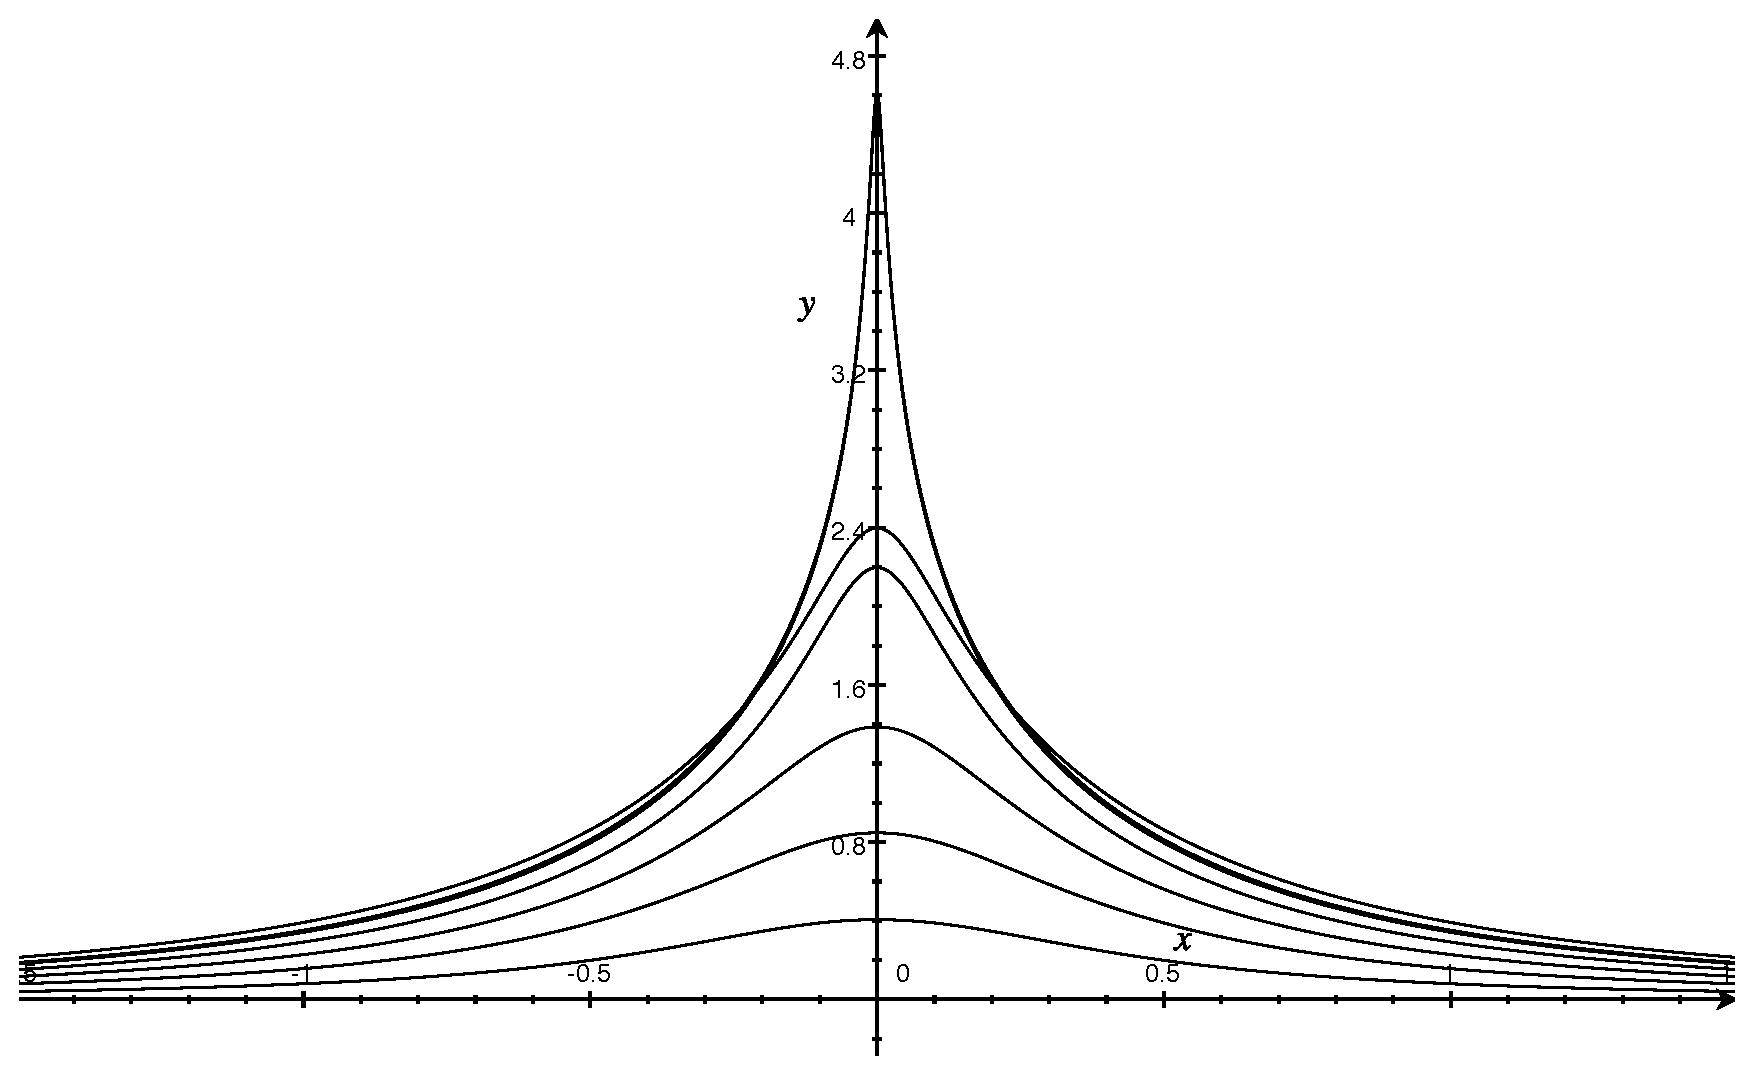
\includegraphics[width=0.48\linewidth]{Figs/Grapher/ModelGreen/reg.eps}
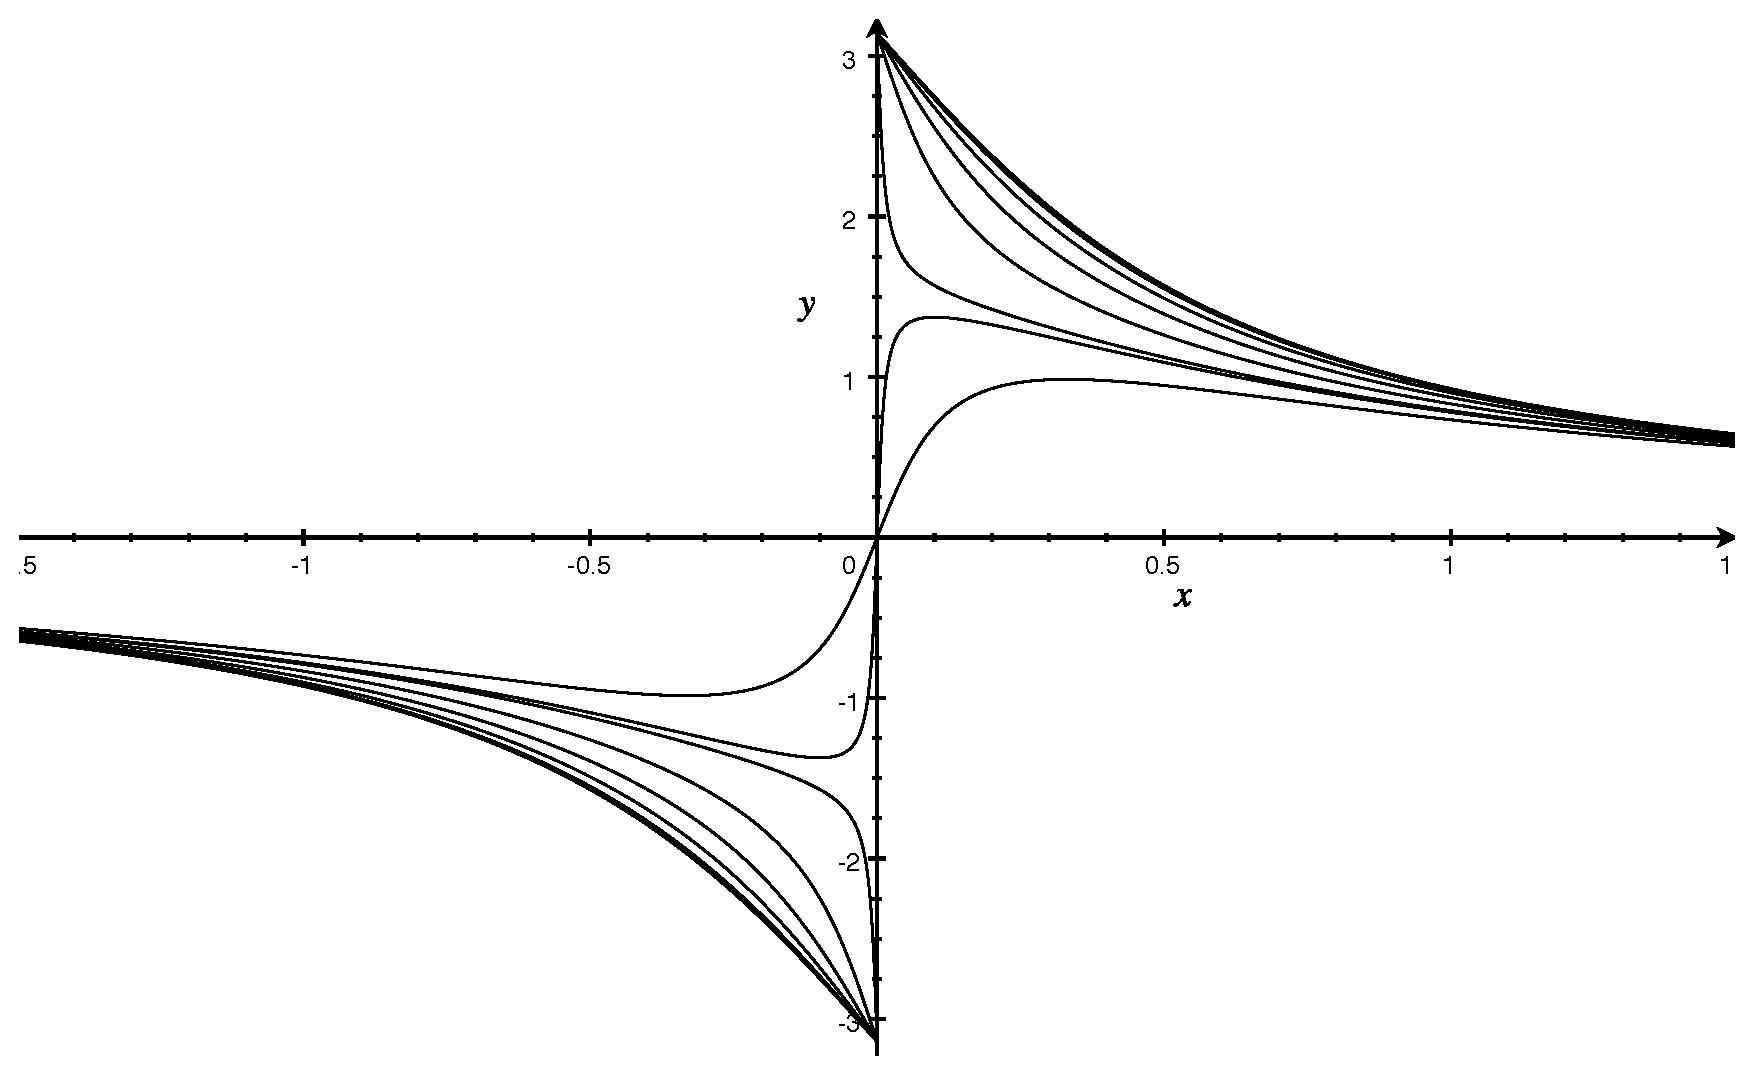
\includegraphics[width=0.48\linewidth]{Figs/Grapher/ModelGreen/img.eps}
\end{center}
\caption{\label{fig:modelgreen}Negative real part (left) and negative imaginary
  part (right) of the Greens function with a constant density of
  states of width $W=1$, centered at
  $E=\{0,0.1,0.2,0.3,0.49,0.51,0.6\}$.}
\end{figure}
The real part is symmetric about
the origin, while the imaginary part is antisymmetric. This is
consistent with $\mat{G}(-i\omega_\nu)=\mat{G}^\dagger(-i\omega_\nu)$.

The imaginary part exhibits a
step at the origin from $\pi/W$ to $\pi/W$ for metallic systems, that is
for a finite density of states at the origin.  For an insulating
system the imaginary part of the Green's function is smooth and has a
finite slope at the origin. 

The real part is positive if the band is
centered above the chemical potential and it is negative if it is
centered below. The real part vanishes if the density of states at the
Fermi level. The real part becomes spiky exactly when the band
touches the Fermi level. As the density of states shifts further to
positive energies, the Greens function grows further in the tails, but
it shrinks in the central region.


\petertt{The following is not correct! Please check!}

Limiting cases
\begin{itemize}
\item $\hbar\omega\rightarrow 0$:

We use the expansion of the arcus tangens
\footnote{
\begin{eqnarray}
  atan(x)&=&y\quad\Rightarrow\quad y=tan(x)=\frac{\sin(x)}{\cos(x)}
\nonumber\\
x&=&\frac{1}{\frac{\pi}{2}-y}+O(y-\frac{\pi}{2})^2
\quad\Rightarrow\quad 
y\approx\frac{\pi}{2}-\frac{1}{x}\quad\text{for $x\rightarrow+\infty$}
\nonumber\\
x&=&\frac{1}{y+\frac{\pi}{2}}+O(y+\frac{\pi}{2})^2
\quad\Rightarrow\quad 
y\approx-\frac{\pi}{2}+\frac{1}{x}\quad\text{for $x\rightarrow-\infty$}
\end{eqnarray}
} and the expanion of the logarithm
\footnote{
\begin{eqnarray}
\ln\left[\frac{a+x}{b+x}\right]\approx
\ln\left[\frac{a}{b}\right]+\left(\frac{1}{a}+\frac{1}{b}\right)x+O(x^2)
\end{eqnarray}
}.
\begin{eqnarray}
G_{a,b}(i\omega_\nu)&=&
\frac{\delta_{a,b}}{W}
\biggl\lbrace
+\frac{1}{2}\ln\left[
\frac{(\hbar\omega)^2+(E-W/2)^2}{(\hbar\omega)^2+(E+W/2)^2}
\right]
-i \left[\atan\left(\frac{E+W/2}{\hbar\omega}\right)
-\atan\left(\frac{E-W/2}{\hbar\omega}\right)\right]
\biggr\rbrace
\nonumber\\
%
&\approx&
\frac{\delta_{a,b}}{W}
\biggl\lbrace
+\frac{1}{2}\ln\left[\left(
\frac{(E-W/2)}{(E+W/2)}\right)^2
\right]
+\frac{1}{2}\left[\frac{1}{(E-W/2)^2}-\frac{1}{(E+W/2)^2}\right]\hbar\omega^2
\nonumber\\
&&-i \left[\frac{\pi}{2}-\frac{\hbar\omega}{E+W/2}
\underbrace{
-\frac{\pi}{2}+\frac{\hbar\omega}{E-W/2}
}_{\text{times -1 for insulators}}\right]
\biggr\rbrace
\nonumber\\
%
&\approx&
\frac{\delta_{a,b}}{W}
\biggl\lbrace
+\ln\left[
\frac{(E-W/2)}{(E+W/2)}
\right]
+\frac{EW}{\left(E^2-\left(\frac{W}{2}\right)^2\right)^2}\hbar\omega^2
-i 
\begin{cases}
\frac{W}{E^2-\left(\frac{W}{2}\right)^2}\hbar\omega
&\text{for insulators}\\
\pm\pi-\frac{4|E|}{E^2-\left(\frac{W}{2}\right)^2}\hbar\omega
&\text{for metals}\\
\end{cases}
\hspace{0.3cm}\biggr\rbrace
\nonumber\\
\end{eqnarray}
%
\item $\hbar\omega\rightarrow \infty$:
\begin{eqnarray}
G_{a,b}(i\omega_\nu)&=&
\frac{\delta_{a,b}}{W}
\biggl\lbrace
+\frac{1}{2}\ln\left[
\frac{(\hbar\omega)^2+(E-W/2)^2}{(\hbar\omega)^2+(E+W/2)^2}
\right]
-i \left[\atan\left(\frac{E+W/2}{\hbar\omega}\right)
-\atan\left(\frac{E-W/2}{\hbar\omega}\right)\right]
\biggr\rbrace
\nonumber\\
%
&\approx&
\frac{\delta_{a,b}}{W}
\biggl\lbrace
-EW(\hbar\omega)^{-2}
-i W (\hbar\omega)^{-1}
\biggr\rbrace
%
\nonumber\\
&\approx&
\delta_{a,b}
\biggl\lbrace
-E(\hbar\omega)^{-2}
-i  (\hbar\omega)^{-1}
\biggr\rbrace
\end{eqnarray}
\end{itemize}


Remark: We can approximate
\begin{eqnarray}
\frac{1}{G_{a,a}^2}\approx \left(
\frac{1}{W}\ln\left[\frac{E-W/2}{E+W/2}\right] \right)^{-2}
  +(\hbar\omega)^2
\end{eqnarray}

%==============================================================================
\section{Preconditioning}
%==============================================================================
With this model and using $E=0$ we obtain
\begin{eqnarray*}
\ddot{\Sigma}_{a,b}(i\omega_\nu)
&=&
\frac{1}{m_\Sigma(\omega_\nu)}
\sum_{c,d}
G^{corr}_{a,c}(i\omega_\nu)
\biggl[\Sigma_{c,d}(i\omega)
-\frac{\beta\partial \Phi^{LW}}{\partial{G}^{loc}_{d,c}(i\omega_\nu)}
\biggr]
G^{corr}_{d,b}(i\omega_\nu)
\nonumber\\
&=&
\frac{1}{m_\Sigma(\omega_\nu)}
\sum_{c,d}
\biggl[-i\delta_{a,c} \frac{1}{W/2}\atan(\frac{W/2}{\hbar\omega})\biggr]
\biggl[\Delta\Sigma_{c,d}(i\omega)
-\frac{\beta\partial \Delta\Phi^{LW}}{\partial{G}^{loc}_{d,c}(i\omega_\nu)}
\biggr]
\nonumber\\
&&
\biggl[-i\delta_{d,b} \frac{1}{W/2}\atan(\frac{W/2}{\hbar\omega})\biggr]
\nonumber\\
&=&
-\frac{1}{m_\Sigma(\omega_\nu)}
\left(\frac{\atan(\frac{W/2}{\hbar\omega})}{(W/2)}\right)^2
\biggl[\Delta\Sigma_{a,b}(i\omega)
-\frac{\beta\partial \Delta\Phi^{LW}}{\partial{G}^{loc}_{b,a}(i\omega_\nu)}
\end{eqnarray*}

Thus we make the ansatz for the $\omega$-dependent mass for the self energy as
\begin{eqnarray}
m_\Sigma(\omega_\nu)=A\left(\frac{\atan(\frac{W/2}{\hbar\omega})}{(W/2)}\right)^2
\end{eqnarray}
where $A$ is a parameter.
For $\omega\rightarrow\infty$ the mass approaches
$A/(\hbar\omega)^2$. Near the origin, however the mass does not
vanish, but it approaches a constant, namely
$A(\frac{\pi}{W})^2$.

Let us define two parameters that determine the $\omega$-dependent mass.
\begin{eqnarray}
M_\Sigma&=&m_\Sigma(0)
\\
C_\Sigma&=&\lim_{\omega\rightarrow\infty} m_\Sigma(\omega)\cdot(\hbar\omega)^2
\end{eqnarray}

With these parameters we obtain
\begin{eqnarray}
m_\Sigma(\omega_\nu)\approx M_\Sigma
\biggl[
\frac{2}{\pi}
\atan\Bigl(\frac{\pi}{2}
\sqrt{\frac{C_\Sigma}{M_\Sigma}}\frac{1}{\hbar\omega}\Bigr)
\biggr]^2
\end{eqnarray}

An approximation for the mass \petertt{(which is not used, though!)} is
\begin{eqnarray}
m_\Sigma(\omega_\nu)\approx m_\Sigma
\biggl[\Bigl(\frac{2}{\pi W/2}\Bigr)^2+(\hbar\omega)^2\biggr]^{-1}
=C_\Sigma
\biggl[\frac{C_\Sigma}{M_\Sigma}+(\hbar\omega)^2\biggr]^{-1}
\end{eqnarray}
which has the same value at the origin and the same tail for
$\omega\rightarrow\infty$. At the origin it does not have the kink of
the original function but remains larger.

The mass for the low frequency region is $M_\Sigma$ and the mass of
the high-frequency region is $C_\Sigma/(\hbar\omega)^2$.  The
high-frequency tail of the Greens function is system independent,
which allows us to determine a canonical value for $C_\Sigma$, that
only depends in the time step. If the period of the high-frequency
tail shall be 10 time steps, $C_\Sigma$ should have the value
$C_\Sigma=\left(\frac{10\Delta t}{2\pi}\right)^2=$, which is about 250
for $\Delta t=10$.

If the period is fixed, we can determine also the optimum friction as
$a_{opt}=\frac{\alpha_{opt}}{2}\Delta t=2\pi\frac{\Delta t}{T}$ which
is with our choices $a_{opt}=\frac{2\pi}{10}$. It is not adviseable
tio choose such a factor, because it would overdamp the low-frequency
region.



%% %=============================================================
%% \subsubsection{Problems:}
%% %=============================================================
%% \begin{itemize}
%% \item the density matrix obtained from the Matsubara sum has
%%   eigenvalues that lie beyond the interval $[0,1]$. Tests for
%%   Matsubara sums hower shows that the spectrum of occupations should
%%   be smaller for a finite sum that that the true result.
%% %
%% \item for a given self energy the density-matrix constraint may not be
%%   fulfillable. 
%% %
%% \item If we set $\Gamma$ and $Y^{(2)}$ to zero, the optimization of the
%%   self energy is almost decoupled from that of the density matrix.

%% Thus we may consider to replace the equation of motion for the
%% Lagrange multipliers by a discrete transformation.
%% \end{itemize}

%% %=============================================================
%% \newpage
%% \subsection{Linear stability analysis}
%% %=============================================================
%% It is not clear if these dynamical equations approach a fix point if a
%% friction is applied. The reason is (1) that it is not proven that the
%% functional is a minimum with respect to the self energy and (2) the
%% dynamics for the constraint equation is not derived from a minimum
%% principle.

%% The two problematic cases are related to self energy and Lagrange
%% multipliers. Therefore we should analyze the dynamics within this
%% subspace for a fixed one-particle density matrix. In order to
%% understand the dynamics we do a linear stability analyses about a
%% fixed point.

%% We linearize $\bar{\mat{\rho}}$ \eq{eq:defrhobar} about the equilibrium
%% self energy. For the second differential equation, we use
%% \eq{eq:quantityxforderivatives} and expand about $\mat{Y}=0$, with $Y$
%% defined in \eq{eq:defbigy}.
%% \petertt{In the following there is a mixup with $\beta$'s!!}

%% \begin{eqnarray}
%% m_\Gamma\delta\ddot{\Gamma}_{n,n'}
%% &=&\frac{1}{\beta}\sum_\nu\sum_{a,b}
%% \underbrace{
%% \Bigl[
%% \sum_{m,m'} G_{n,m}(i\omega_\nu)\langle\psi_m|\bar{\pi}_a\rangle
%% \langle\bar{\pi}_b|\psi_{m'}\rangle G_{m',n'}(i\omega_\nu)\Bigr]
%% }_{B_{b,a,n',n}(i\omega_\nu)}
%% \delta\Delta\Sigma_{a,b}(i\omega_\nu)
%% \nonumber
%% \\
%% m_\Sigma\delta\Delta\ddot{\Sigma}_{a,b}(i\omega_\nu)
%% &=&\sum_{n,n'}\underbrace{
%% \Bigl[\sum_{m,m'}
%% \langle\bar{\pi}_a|\psi_{m}\rangle G_{m,n}(i\omega_\nu)
%% G_{n',m'}(i\omega_\nu)\langle\psi_{m'}|\bar{\pi}_b\rangle
%% \Bigr]}_{B_{a,b,n,n'}(i\omega_\nu)}\delta\Gamma_{n,n'}
%% \end{eqnarray}

%% After a Fourier ttransform in time we obtain the following matrix equation
%% \begin{eqnarray}
%% \left(\begin{array}{cccc}
%% \beta m_\Gamma\omega^2 & B^{\dagger,\dagger}(i\omega_1) 
%%                 & B^{\dagger,\dagger}(i\omega_2) &\ldots\\
%% B(i\omega_1) & m_\Sigma\omega^2 & 0 & \ldots\\
%% B(i\omega_2) & 0&m_\Sigma\omega^2 &  \ldots\\
%% \vdots &\vdots & 0 & 
%% \end{array}\right)
%% \left(\begin{array}{c}
%% \Gamma \\ \Sigma(i\omega_1)\\ \Sigma(i\omega_2) \\ \vdots
%% \end{array}\right)
%% =0
%% \end{eqnarray}
%% From the lower equation, we obtain
%% \begin{eqnarray}
%% \Sigma(i\omega_\nu)=\frac{1}{m_\Sigma\omega^2}B(i\omega_\nu)\Gamma
%% \end{eqnarray}
%% which we insert into the uppermost equation
%% \begin{eqnarray}
%% &&\Bigl[m_\Gamma\omega^2-\sum_\nu B^{\dagger,\dagger}(i\omega_\nu) 
%% \frac{1}{m_\Sigma\omega^2}B(i\omega_\nu)\Bigr]\Gamma=0
%% \nonumber
%% \\
%% &&\sum_{p,p'}\biggl\lbrace
%% m_\Gamma\omega^2\delta_{n,p}\delta_{n',p'}
%% -\frac{1}{\beta}\sum_{\nu}
%% \sum_{a,b}\Bigl[
%% \sum_{m,m'} G_{n,m}(i\omega_\nu)\langle\psi_m|\bar{\pi}_a\rangle
%% \langle\bar{\pi}_b|\psi_{m'}\rangle G_{m',n'}(i\omega_\nu)\Bigr]
%% \nonumber\\
%% &&\hspace{3cm}\cdot
%% \frac{1}{m_\Sigma\omega^2}
%% \Bigl[\sum_{m,m'}
%% \langle\bar{\pi}_a|\psi_{m}\rangle G_{m,p}(i\omega_\nu)
%% G_{p',m'}(i\omega_\nu)\langle\psi_{m'}|\bar{\pi}_b\rangle
%% \Bigr]
%% \biggr\rbrace\Gamma_{p,p'}=0
%% \nonumber
%% \\
%% \Rightarrow&&\sum_{p,p'}\biggl\lbrace
%% m_\Gamma m_\Sigma \omega^4\delta_{n,p}\delta_{n',p'}
%% -
%% \frac{1}{\beta}\sum_{\nu}
%% \Bigl[
%% \sum_{a,m,q}G_{n,m}(i\omega_\nu)\langle\psi_m|\bar{\pi}_a\rangle
%% \langle\bar{\pi}_a|\psi_{q}\rangle G_{q,p}(i\omega_\nu)\Bigr]
%% \nonumber\\
%% &&\hspace{3cm}\cdot
%% \Bigl[\sum_{b,m',q'}
%% G_{p',q'}(i\omega_\nu)\langle\psi_{q'}|\bar{\pi}_b\rangle
%% \langle\bar{\pi}_b|\psi_{m'}\rangle G_{m',n'}(i\omega_\nu)\Bigr]
%% \biggr\rbrace\Gamma_{p,p'}=0
%% \end{eqnarray}
%% This equation factorizes according to the Bloch vectors.

%% The physical meaning of 
%% \begin{eqnarray}
%% \sum_{b,m',q'}
%% &&G_{p',q'}(i\omega_\nu)\langle\psi_{q'}|\bar{\pi}_b\rangle
%% \langle\bar{\pi}_b|\psi_{m'}\rangle G_{m',n'}(i\omega_\nu)
%% \\
%% &=&\left.\frac{d}{dV}\right|_{V=0}
%% \Bigl[\Bigl(\mat{G}(i\omega_\nu)\Bigr)^{-1}_{n',p'}
%% -\sum_{a,b}\langle\psi_{n'}|\bar{\pi}_a\rangle V\delta_{a,b}
%% \langle\bar{\pi}_b|\psi_{p'}\rangle
%% \Bigr]^{-1}_{p',n'}
%% \end{eqnarray}
%% is that of the response of the Green's function to a constant external
%% potential acting on the orbitals in the correlated subspace.

%% This dynamics is unstable. The forces point in the angular direction
%% and increase with the distance from the center. Thus the centrifugal
%% force shifts the dynamics to increasingly larger orbits.
%% \begin{center}
%% {\tiny
%% \begin{verbatim}
%%        program dyn
%%        implicit none
%%        integer(4),parameter :: niter=10000
%%        real(8)   ,parameter :: dt=1.d0
%%        real(8)   ,parameter :: m=-1.d0
%%        real(8)   ,parameter :: anne=5.d0
%%        real(8)   ,parameter :: c1=1.d0,c2=-1.d0
%%        integer(4)           :: iter
%%        real(8)              :: x0(2),xp(2),xm(2),f(2)
%% !      *************************************************************************
%%        x0=(/1.d0,0.d0/)
%%        xm=x0
%%        do iter=1,niter
%% !        == write ========================
%%          write(*,fmt='(i5,2e20.5)')iter,x0
%% !        == forces ======================
%%          f(1)=-c1*x0(2)
%%          f(2)=-c2*x0(1)
%% !        == propagate
%%          xp=(x0*2.d0-xm*(1.d0-anne)+f*dt**2/m)/(1.d0+anne)
%% !        == switch
%%          xm=x0
%%          x0=xp
%%       enddo
%%       stop
%%       end
%% \end{verbatim}}
%% \end{center}

%% Conceivable is to fix the self energy and allow the density matrix to
%% adjust, including the Lagrange parameters. The Lagrange parameters act
%% as forces for an outer loop in which the self-energy is optimized.




%==============================================================================
\section{Bloch representation}
%==============================================================================



\clearpage
\bibliographystyle{unsrtnat} 
 \bibliography{../all}
\end{document}  
 
